\documentclass{article}

%----------------------------------------------------------------------------------------
%	PACKAGES AND OTHER DOCUMENT CONFIGURATIONS
%----------------------------------------------------------------------------------------

\usepackage[T1]{fontenc}
\usepackage[utf8]{inputenc}
\usepackage{lmodern}
\usepackage[english]{babel}
\usepackage[autostyle]{csquotes}
\usepackage{graphicx} % Required for inserting images
\usepackage[hyphens]{url}
\usepackage{hyperref}
\usepackage{amsmath}      % for additional mathematical features
\usepackage{amsfonts}     % for mathbb command
\usepackage{float}
\usepackage{setspace}
\usepackage{listings}
\usepackage{rotating}
\doublespacing
\usepackage[backend=biber,style=authoryear]{biblatex}
\renewcommand*{\bibfont}{\small}
\addbibresource{Bibliography.bib}
\usepackage{tcolorbox}
\usepackage{amssymb}

%----------------------------------------------------------------------------------------
%	DOCUMENT MARGINS
%----------------------------------------------------------------------------------------

\usepackage{geometry} % Required for adjusting page dimensions and margins

\geometry{
	paper=a4paper, % Paper size, change to letterpaper for US letter size
	top=3cm, % Top margin
	bottom=3cm, % Bottom margin
	left=3cm, % Left margin
	right=3cm, % Right margin
	headheight = 10pt, % Header height
	footskip = 1.5cm, % Space from the bottom margin to the baseline of the footer
	headsep = 1.2cm, % Space from the top margin to the baseline of the header
	%showframe, % Uncomment to show how the type block is set on the page
}

%----------------------------------------------------------------------------------------
%	SECTION TITLE APPEARANCE
%----------------------------------------------------------------------------------------


\title{Diversity as a management tool for forest ecosystem services \\ 
\large A theoretical exploration using control theory and viability analyses}
\author{Clementine de Montgolfier}
\date{Dec 2023}

\begin{document}

\begin{titlepage}
    \begin{center}
        
        \Huge
        \textbf{Diversity as a management tool for forest ecosystem services}
 
        \LARGE
        A theoretical exploration using control theory and viability analyses
             
        \vspace{0.5cm}

        \Large  
        \textbf{Clémentine de Montgolfier}

        \large  
        Ecole Normale supérieure\\
        February 2024

        \vspace{0.5cm}
        
        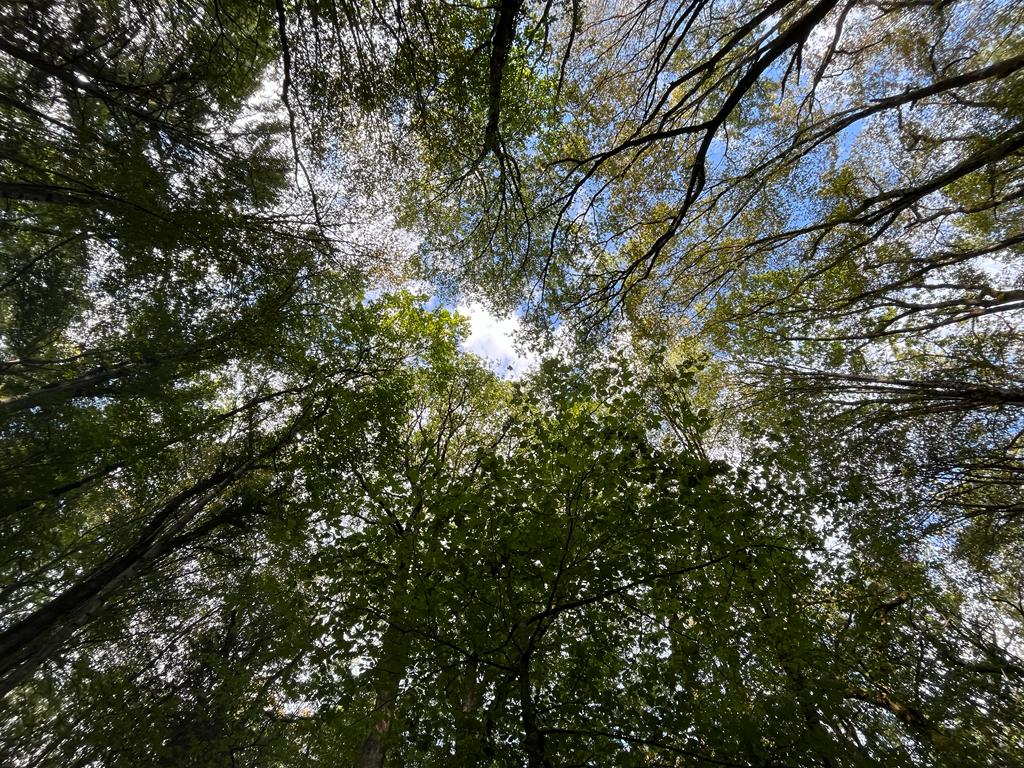
\includegraphics[height=8cm]{Figure/forest.jpg}

        \vspace{0.5cm}

        \large
        At the LISC laboratory (INRAE)\\
        Under the supervision of Jean-Denis Mathias, Marion Jourdan and Jean-Baptiste Pichancourt

        % Bottom Logos
        \begin{minipage}[b]{0.5\textwidth}
            \vspace{1cm}
            
\includegraphics[height=2.2cm]{Figure/ENS_logo.png}
        \end{minipage}%
        \begin{minipage}[b]{0.5\textwidth}
            \hfill
            
\includegraphics[height=1.4cm]{Figure/INRAE_logo.png}
        \end{minipage}

    \end{center}
\end{titlepage}

\pagenumbering{Roman}

\section*{Abstract}

Defining optimal forest management strategies in a changing world is a challenge in the field of forest ecology. The complexity of forest ecosystems, coupled with the uncertainty of future climate conditions, makes it difficult to determine the best course of action. The concept of forest diversity is a key consideration in this debate, as it is believed to be a significant factor in the resilience of forest ecosystems. This study aims to explore whether diversity can be used as a management tool to maintain the ecosystem in a desirable state. To this end, we will use a theoretical model of a mixed-species, multi-layered forest, and apply control theory and viability analyses to assess the relationship between diversity and management trajectories, considering both species and vertical diversity at the stand level. RESULTS\\

\noindent \textbf{Keywords:} forest management, diversity, control theory, viability theory

\newpage

\section*{Acknowledgement}

Je voudrais remercier tout d'abord mes encadrant.e.s, Marion, Jean-Denis et Jean-Baptiste pour m'avoir accompagnée tout au long de ce stage. Merci pour tout vos retours sur mon travail, votre disponibilité et votre patience. Merci pour les conseils et les pistes de réflexion. J'ai beaucoup aimé travailer avec ces trois regards complémentaires sur le sujet.

Merci Marion pour les deux semaines passées à Nancy qui nous ont permis de faire un point sur l'aspect pratique du stage et d'apprendre enfin à jouer au go.

Ammar ça a été un plaisir de partager mon bureau avec toi, je te souhaite plein de courage pour ton premier papier et la suite de ta thèse. Merci beaucoup Michelle aussi pour ta présence au labo et pour les ballades dans les puys. Louise tu es arrivée tard dans mon stage mais ça a été très chouette de te croiser au LISC. Merci à tous les membres de l'équipe pour les pauses cafés et les discussions.

Mon stage n'aurait pas été le même sans mes collocs. Valentine, Yoann, Gabriel, Julie et Malek, merci (Lilith et Callipso je ne vous oublie pas). Je me suis senti chez moi chez nous. Les parties de Mario kart ont été mémorables. Si j'ai la chance de revenir il va falloir que je trouve un moyen de maintenir le niveau dans l'interval.

\newpage

\begin{singlespace}
    \tableofcontents
\end{singlespace}

% skip page
\newpage

\pagenumbering{arabic}

\section{Intro}

\subsection{Forest and management, new practices for new challenges}

Forest covers 31\% of the territory in France, however forest health metrics show rapid degradation  marked by an alarming +80\% increased mortality rate, a 4\% decline in growth and a deceleration in carbon storage due to the growing number of health crises combined with more frequent droughts ~\autocite{IGN}. This impacts forest composition, structure, dynamics and the provisioning of ecosystem services to human populations (Climate regulation, water purification, wood production, air quality, cultural leisure...) ~\autocite{grammatikopoulouValueForestEcosystem2021}. Notably, 94\% of these forests are designated as productive, emphasizing the critical need to adapt management strategies to address these emerging challenges. 
New adaptative policy actions are studied to robustly sustain the state of these forests as the adaptation from monospecific forets stand with clear-cutting into mixed species and uneven aged forest stand with a diversity of selectives logging practices  ~\autocite{raymondIrregularShelterwoodSystem2009}. Knowledge of these nexw practices is still limited but they are already implemented relying on the idea that diversification is a way to increase multiple ecosystem services ~\autocite{tilmanBiodiversityPopulationEcosystem1996}.

For obvious economic constraints sustainable wood extraction has been the primary driver of forest management practices. With this approach diversity indices are treated as auxiliary metrics, preventing interference with the core objective of wood extraction. The pivotal question that emerges is whether we can redefine this paradigm and choose diversity as our primary constraints to explore potential benefits and differences in our management approaches.This paradigm shift is motivated, firstly, by the insights from Biodiversity-Ecosystem Functioning (BEF) studies, which highlight diversity as a critical component for overall ecosystem health. Our study's second motivation is the indicating that forest management can function as a tool to actively enhance diversity within ecosystems. But given the many uncertainties in climate and the complex response of forest systems to management actions, new methods (using models and decision science) are needed to assist their design.

\subsection{Diverstity and ecosystem functionning}

Work on composition diversification and its effects is mainly driven by the first work on BEF from grassland studies ~\autocite{tilmanBiodiversityPopulationEcosystem1996} showing a positive link between biodiversity and ecosystem functioning. But even though numerous hypothesis were made to explain this link (competitive exclusion, niche complementary, sampling effect, etc.) the mechanisms behind this link are still not well understood ~\autocite{aliBiodiversityEcosystemFunctioning2023}. This uncertainty makes it difficult to predict the impact of biodiversity loss.
While the hypothesis of BEF relationship, and its relevance is still debated, it fuels an entire segment of research.
In forest, the study of BEF is more recent and mainly focused on the link between species diversity and productivity. A positive relationship has been demonstrated at a global scale ~\autocite{liangPositiveBiodiversityproductivityRelationship2016}, but also in specific forest ~\autocite{morinTreeSpeciesRichness2011,paquetteEffectBiodiversityTree2011,jourdanManagingMixedStands2021}. But the interaction is not positive in every forest type. ~\autocite{forresterReviewProcessesDiversity2016}.
This may suggest that the biodiversity-productivity interaction is context dependant, the relationship seems to be mostly positive in harsh climate and low tree density but negative in suitable environment ~\autocite{juckerClimateModulatesEffects2016}.

It is also reductive to consider productivity as the only function of forest ecosystems, and other should be accounted for: flora and fauna biodiversity, carbon storage, water and biochemical cycle that provide multiple services to human populations ~\autocite{aertsForestRestorationBiodiversity2011}.
To gain a comprehensive understanding of the diverse impacts of biodiversity on forest functioning, it is essential to simultaneously investigate multiple functions, as they may not be affected in uniform ways ~\autocite{korboulewskyHowTreeDiversity2016}. It introduces a level of complexity not observed when studying individual functions like the jack-of-all-trades and master of none mechanism ~\autocite{vanderplasJackofalltradesEffectsDrive2016} blindly increasing biodiversity can increase forest multi-functionnality without optimizing any of them and leading sometimes to trade-offs. It is thus important to define the functions that we want to preserve as well as threshold for each of them. 
Forests exhibit different functions not solely tied to species identity but also emerging from distinct life stages within the same species. Noteworthy tade-offs can be observed in the comparison between young and old grown forests, if the former are more productive, they store less carbon than the latter ~\autocite{caspersenSuccessionalDiversityForest2001}. Recognizing the diverse advantages of both young and old forests could involve reintroducing vertical diversity through uneven forest management l to enhance overall ecosystem resilience and functionality ~\autocite{guldinRoleUnevenAgedSilviculture1996}. However, despite its promise, the implementation of such practices remains limited, with only 25\% of managed forests in Europe currently comprising uneven-aged stands (foresteurope.org).
This limitation is accentuated by a notable gap in our understanding of the ecological consequences of uneven-aged stages within forest ecosystems. The complex interplay of factors makes it challenging to draw definitive conclusions regarding the comparative ecological effects of even-aged and uneven-aged silviculture ~\autocite{noletComparingEffectsEven2018}. Consequently, the full scope of benefits and potential drawbacks associated with fostering vertical diversity in forest management is not yet well comprehended. This dual challenge of limited implementation and incomplete understanding underscores the importance of further research to inform and refine forest management practices.
Even if the advantages of diversity in forests are convincingly demonstrated, implementing management strategies to promote it is no straightforward task. This requires a profound understanding of forest dynamics and the short, medium, and long-term responses to interventions within the forest ecosystem.

\subsection{Mangement for diversity}

While diversity is not always a priority in forest management— with a significant portion (1/3) of forests in Europe still mono-specific and the majority (3/4) being even-aged (foresteurope.org) various practice philosophies have been proposed to reintroduce diversity into managed forests. Two prominent approaches include retention forestry and the irregular shelterwood system.
Retention forestry aims to maintain forest structure and composition by leaving a certain proportion of trees in the stand after harvesting ~\autocite{gustafssonRetentionForestryMaintain2012,rosenvaldWhatWhenWhere2008}. Similarly, the irregular shelterwood system, also known as uneven-aged forestry or continuous cover forestry, focuses on sustaining a continuous cover of trees in the stand, promoting both structural and vertical diversity ~\autocite{sinhaOptimalManagementNaturally2017,schallImpactEvenagedUnevenaged2018,nylandEvenUnevenagedChallenges2003,noletComparingEffectsEven2018,dudumanForestManagementPlanning2011}. However, a notable gap exists in the understanding of the long-term dynamics and consequences of these practices, with limited predictive studies on system dynamics.

On the other hand theoretical ecology, studies species coexistence providing insights into enhancing diversity by controlling various aspects of the forest ecosystem ~\autocite{wilsonTwelveTheoriesCoexistence2011}. The intermediate disturbance hypothesis, for example, suggests that maintaining intermediate levels of disturbance allows for the coexistence of species with different disturbance tolerances ~\autocite{connellDiversityTropicalRain1978,sheilDefiningDefendingConnell2013}. Another strategy involves cutting dominant species to promote the development of other species ~\autocite{pichancourtGrowingBiodiverseCarbonrich2014}.
Despite these approaches offering valuable insights into managing biological diversity, challenges persist. The applicability of these theories to real-world forest management scenarios is limited, and they face contestations within the scientific community ~\autocite{mackeyReexaminationExpectedEffects2000,foxIntermediateDisturbanceHypothesis2013}.

These studies emphasize the need for a comprehensive understanding of forest management beyond traditional cutting practices. They strive to provide guidance for managing biological diversity thanks to different management practices. However extracting an optimal management trajectory proves challenging due to the current limitations in our understanding, coupled with the added complexity of simultaneously maximizing multiple ecological functions. Exploring the possibility of new forest management focused on mitigating drawbacks on diversity and not optimisation could open new perspectives.\\

\subsection{Hypothesis and objectives of the study}

Given the understanding that diversity holds significance for optimal forest functioning and recognizing management as a pivotal tool in shaping this diversity, our main hypothesis is that using diversity as a constraints for management instead of productivity could bring forth new management strategies. To test this, we developed a simple theoretical model of multi-species/layers forest ecosystem dynamics. The model was parameterized for two species with different vital rates (growth, survival, reproduction) and competition for light between three vertical storeys (upper, mid, under). The model was used to predict annual Shannon diversity index of species, vertical structure, above-ground biomass, and timber extraction every ten years.  Algorithm from viability theory were used to deduce the the set of states and controls that respect our constraints. With this approach we where able to compare the management trajectories that respect diversity constraints with the ones that respect wood extraction constraints. 

\section{Methods}

\subsection{Forest model}
 
\subsubsection{Choice of model}

Selecting an appropriate forest model is a critical decision shaped by the inherent complexities of forest ecosystems. They evolved with need, understanding of ecosystem processes, and technological innovations. They are applied at different spacial scales from tree, to stand to landscape level. They integrate various processes as growth, regeneration, mortality, management, photosynthesis, evapotranspiration, disturbances with more or less details and assumptions. Numerous types of forest model classification exist ~\autocite{porteModellingMixedForest2002}. 

One of the main gradient is the classification from empirical to process-based model ~\autocite{fontesModelsSupportingForest2011},  choosing between detailed geometric description and predictive capability for unexplored conditions. The former, rooted in statistical models, excels in predictive power within captured contexts but falls short in addressing novel scenarios. On the other hand, process-based models, exemplified by Gap-models ~\autocite{bugmannREVIEWFORESTGAP2001}, balance this trade-off by inferring dynamics from underlying processes at community,individual or cellular level. The description of macroscopic processes in phenomenological models emphasize simplicity using forest-level variables. These models provide analytical solutions and support sensitivity analyses but necessitate frequent re-parametrization to accommodate diverse contexts. Conversely, mechanistic models, detailing microscopic models, rooted in the fundamental principles of tree biology, integrate numerous variables for universal adaptability. Nevertheless, the analytical intricacy of these models imposes limitations on exploring model boundaries through sensitivity analyses ~\autocite{bugmannREVIEWFORESTGAP2001}.

In theoretical forest modeling, attempts have been made to bridge the gap between phenomenological and mechanistic models. This can be pursued by applying methodological progress as mean-field approaches or aggregation methods to reduce dimensions while making minimal assumptions like  with DisCForM and TreeMig ~\autocite{lischkeAggregationIndividualTrees1998,lischkeTreeMigForestlandscapeModel2006} aggregated from ForClim ~\autocite{bugmannEcologyMountainousForests1994}.The goal is to use the parameters of microscopic processes to directly describe the macroscopic dynamic using a limited number of equations.
Both this approach and cohort based model show a remarkable congruence in their formulation ~\autocite{bugmannREVIEWFORESTGAP2001}. However, as of now, neither has demonstrated decisive advancements suitable for practical implementation in solving forest management problems.

Based on the viability analyses we want to perform and its computational cost, the model had to be simple enough to be sumarized by a small number of state variables. But to answer our question it must also allow to test different management strategies for different combinations of species and canopy vertical structure. This led us to choose a deterministic density-based model. We hypothesize that we can use a simple theoretical model to explore the effect of diversity on ecosystem services, and that the some methods and results will then be transferable to process-based models. The advantages of this approach is that we can explore a large range of possibilities and test new hypothesis that could not be tested otherwise.

The model that best fit our criteria is based on the work of Kohyama and associates ~\autocite{kohyamaStratificationTheoryPlant2009, kohyamaOnesidedCompetitionLight2012}. Its structure is described below.

\subsubsection{Model description}

The theoretical model described below comes from the study of multiple articles from Kohyama and associates ~\autocite{kohyamaStratificationTheoryPlant2009, kohyamaOnesidedCompetitionLight2012}.
It is a compartment based model with multi species and multi layers structure Figure ~\ref{fig:fig_model}. The dynamic is influenced by growth, regeneration, mortality as well as competition for light from the layers above. There are some differences between the models present in Kohyama 2009 and 2012, in particular definition of birth and competition. We chose to define birth as in Kohyama 2009 as a negative linear, or Verhulst function (and not as a negative exponential, or Ricker function in Koyama 2012). The only difference is that birth in our study is concidere on independant from the number of adult tree. Even if Kohyama 2009 propose a way to add competition for resources by layers below, we chose a strictly one-sided competition from the above layers as in Kohyama 2012.

\begin{figure}[h]
    \centering
    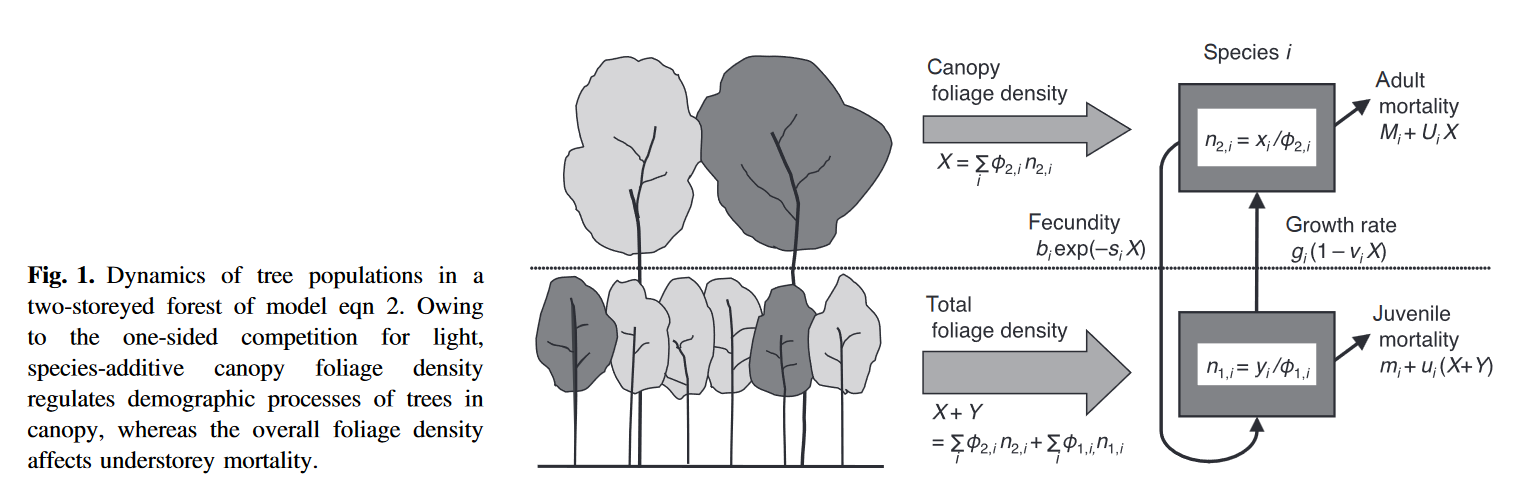
\includegraphics[width=\textwidth]{Figure/Fig_model_Kohyama.png}
    \caption{Figure from ~\autocite{kohyamaOnesidedCompetitionLight2012}}
    \label{fig:fig_model}
\end{figure}

Dynamic of each layer is driven by the competition from above layers foliage density (assimilated to the basal area) $\sum_{i = l}^{L} X_i$ with $X_i$ being the foliage density of layer $i$ defined by the number of tree $n_{sp,i}$ and the mean basal area of tree $\phi_{sp,i}$ of each species ($sp$) in layer $i$:

\begin{equation}
    X_{i} = \sum_{sp} \phi_{sp,i} n_{sp,i}
\end{equation}

The various processes are influenced by competition, with a linear negative relationship. Optimal probabilities are determined for each processes (birth $b$, growth $g$ and mortality $m$) without competition. These probabilities are then adjusted based on the process sensitivity ($Cb$, $Cg$, $Cm$) of the layer and species to foliage density.
The model can be summarised with one equation :

\begin{equation}
\begin{aligned}
    n_{sp,l}(t+1) = {} & n_{sp,l}(t) \\
    & + b_{sp,l} (1 - Cb_{sp,l} \sum_{i = 1}^{L} X_{i}) &&\text{birth} \\
    & + g_{sp,l - 1} \; n_{sp,l-1}(t) (1 - Cg_{sp,l-1} \sum_{i = l-1}^{L} X_{i}) &&\text{growth from lower level}\\
    & - g_{sp,l} \; n_{sp,l}(t) (1 - Cg_{sp,l} \sum_{i = l}^{L} X_{i}) &&\text{growth to upper level}\\
    & - m_{sp,l} \; n_{sp,l}(t) (1 + Cm_{sp,l} \sum_{i = l}^{L} X_{i}) &&\text{mortality} \\
    & - u{sp, l}(t) &&\text{logging}
\end{aligned}
\label{eq:model_general}
\end{equation}

And some special cases for lower and upper layers :

\begin{equation}
\begin{aligned}
    b_{sp,l>1} & = 0 && \text{new trees always arrive in the lower level} \\
    g_{sp,L} & = 0, && \text{trees cannot grow out of the upper layer} \\
    g_{sp,0} & = 0, && \text{trees cannot grow into the lower level} \\
    u_{sp,l<L} & = 0, && \text{we chose to only apply logging to the upper level} \\
    u_{sp,L}(t) = 0 & \text{if} t mod 10 \neq 0 && \text{we chose a discrete cut only applied every ten years} \\ 
\end{aligned}
\label{eq:model_conditions}
\end{equation}

Population densities and demographic parameters are defined in Table ~\ref{tab:coef} and are all positive.

\begin{table}[t]
    \centering
    \begin{tabular}{l l l}
    \hline
    \hline
    \textbf{Abbreviation} & \textbf{Meaning} & \textbf{Unit} \\
    \hline
    \hline
    $l$            & layer index                                                 &          \\
    $L$            & number of layer (i.e. maximum layer)                        &          \\
    $sp$           & species index                                               &          \\
    $SP$           & number of species                                           &            \\
    $n_{sp,l}$     & number of trees of species $sp$ in layer $l$                & $ha^{-1}$  \\    
    $x_{sp,l}$     & foliage density of species $sp$ in layer $l$                & $m^2.ha^{-1}$  \\
    $\phi_{sp,l}$     & mean basal area of tree from species $sp$ in layer $l$    & $m^2$  \\
    $X_{l}$        & foliage density of layer $l$                                & $m^2.ha^{-1}$  \\ 
    $\sum_{i = l}^{L} X_{i}$     & foliage density above layer $l$      & $m^2.ha^{-1}$  \\ 
    $b_{sp}$       & optimal birth rate per tree in layer $L$    &  \\
    $Cb_{sp}$      & birth susceptibility to superior foliage density    & $ha.m^{-2}$           \\
    $g_{sp,l}$     & growth susceptibility to superior foliage density           &  \\
    $m_{sp,l}$     & probability of intrinsic mortality           & \\
    $Cg_{sp,l}$    & growth susceptibility to superior foliage density            &   $ha.m^{-2}$  \\
    $Cb_{sp,l}$    & mortality susceptibility to superior foliage density            & $ha.m^{-2}$    \\
    $u_{sp,l}$     & number of trees cut from species $sp$ in layer $l$           & $ha^{-1}$ \\
    \hline
    \hline
    \end{tabular}
    \caption{Parameters for the model}
    \label{tab:coef}
\end{table}

\subsubsection{Model parametrisation}

We are starting with a 3 layers 2 species system with a mixture of possible species : \textit{Abies alba}, \textit{Betula pendula}, \textit{Fagus sylvatica}, \textit{Picea abies}, \textit{Pinus sylvestris}, \textit{Quercus pubescens}. The layers are defined by simplifying the IGN (French National Institute for Geographic and Forestry Information) 4-dimensional wood classification used in national forest inventory into 3 classes : dbh (cm) in [0,22.5] for small wood, [22.5,67.5] for medium and large, and [67.5+[ for very large. We have to define all parameters from the model.

Litterature and ForCEEPS simulations where used to adjust the dynamic of the system on a constant climate. (see appendix on parametrisation ~\autocite{bugmannEcologyMountainousForests1994,morinForestSuccessionGap2021}). Giving the parameters in Table S.\ref{tab:Final_param}.\\
We choose to concentrate our analyses on two species \textit{Abies alba} and \textit{Fagus sylvatica} as their dynamic was the most similar to ForCEEPS (REF to supplementary data) and they can be found together in mixed stand in France.

\subsection{Viability theory for defining management strategies}

There doesn't seem to be any optimal solution to manage such complicated ecosystems, while taking into account their multi-functionality. Some methods, such as viability theory ~\autocite{aubinStochasticViabilityInvariance1990}, have been developed to actively discover sequences of actions sustaining multiple objectives within satisfaction constraints. Viability analyses establishes a framework to define control and states that can be combined to stay in our biological constraints for as long as needed ~\autocite{rougeExtendingViabilityTheory2013}.
Viability theory finds application in scenarios where objectives involve ecosystem services in forest social-ecological systems ~\autocite{mathiasUsingViabilityTheory2015}. In these studies, biodiversity is leveraged to identify viable control sequences, sustaining forest biodiversity and some ecosystem services through timber extraction control.
Nevertheless, it has not yet been employed to comprehend how controlling species diversity and selective cutting targets can lead to viable management trajectories.

Viability theory provides a framework for management of dynamic systems. The challenge lies in finding management strategies (\(u(t)\)) that perpetually keep the system within a space of chosen constraints $K$. Rather than fixating on a single optimal state, the approach is to navigate within a spectrum of acceptable outcomes, preventing irreversible negative impacts.

In our case, the control is discrete and happens every ten years ($\Delta t$), mathematically, this is articulated as a controlled discrete-time dynamic system (described in equation \eqref{eq:model_general}).The control are discrete and only applied every ten years (see cpounditions described in equation \eqref{eq:model_conditions}). The range of feasible control options every ten years is determined by the number of trees that are cut, ensuring that this number remains lower than the quantity present before the cut.

\begin{equation}
     U = \{u \in \mathbb{N}^{SP} \mid \forall sp \in \mathbb{N}_{[1,SP]} \; u_{sp} \leq n_{sp,L}\}
\end{equation}

The resulting viability kernel (Viab(K)), which includes states where a management strategy can keep the system within desirable states, is formally described as:

\begin{equation}
    Viab(K) = \{N_0 \in K \mid\exists U(\cdot), \forall t \in \mathbb{N}_5, N(t) \in K\},
\end{equation}

where \(N_0\) denotes an initial state of the system in our constraints $K$. Within the viability kernel, at least one control strategy $u(\cdot)$ can maintain the system in a desirable state $K$. After the delimitation of the viability kernel all viable controls (\(u_v\)) can be determined and analysed.

To approach the viability kernel we used an algorithm inspired by Saint-Pierre ~\autocite{saint-pierreApproximationViabilityKernel1994}. APPENDIX

To investigate the impact of shifting focus from wood extraction to promoting diversity, we employed two distinct sets of constraints. The first set exclusively targeted wood extraction, with a minimum limit set at 30 m³/ha every two years ~\autocite{IGN}. The second set focused on diversity and combined two metrics. We chose to use the Shannon index ($H = -\sum_{i=1}^{S} p_i \cdot \ln(p_i)$) as a measure of species and vertical diversity, as it is a common metric in ecology and combine information about diversity and evenness. Firstly, for species evenness, we aimed for at least 20\% representation of minority species in the population, translating to a Shannon index equal to or greater than 0.72. Secondly, for vertical evenness, we aspired to maintain an uneven-aged forest by ensuring that the richer layer comprised less than 80\% of the stems, (Shannon vertical index greater than or equal to 0.92).
\\

To analyze the space of possible states, the algorithm employs a discretization approach, dividing all potential states into a grid. Determining the necessary limits involved a dynamic analysis and examination of the phase diagram. We opted to explore all conceivable states within a range of 0 to 200 trees in each layer for every species, setting an additional cap of 600 trees for the lower level (small trees). Considering technical constraints, a grid was defined with 9 points in each dimension (equivalent to a discretization in steps of 25), with an extra 4 points introduced every 100 stems for the lower layer to get to 600. This resulted in an analysis encompassing approximately a million states, with 81 distinct control combinations applicable, yielding a total of 27 million combinations to study.

The computations were executed using R on a machine equipped with 720 gigabytes of RAM and 60 cores. Running for approximately 10 hours, the algorithm produced the viability kernel analysed in the results. Source code is accessible on GitHub at (\href{https://github.com/clem9123/Forest_management_and_viability}). All analyses were conducted using R ~\autocite{Rsoftware}.

\section{Results}

\subsection{Sensibility and Compatibility of the constraints}

%\begin{figure}[h]
%    \centering
%    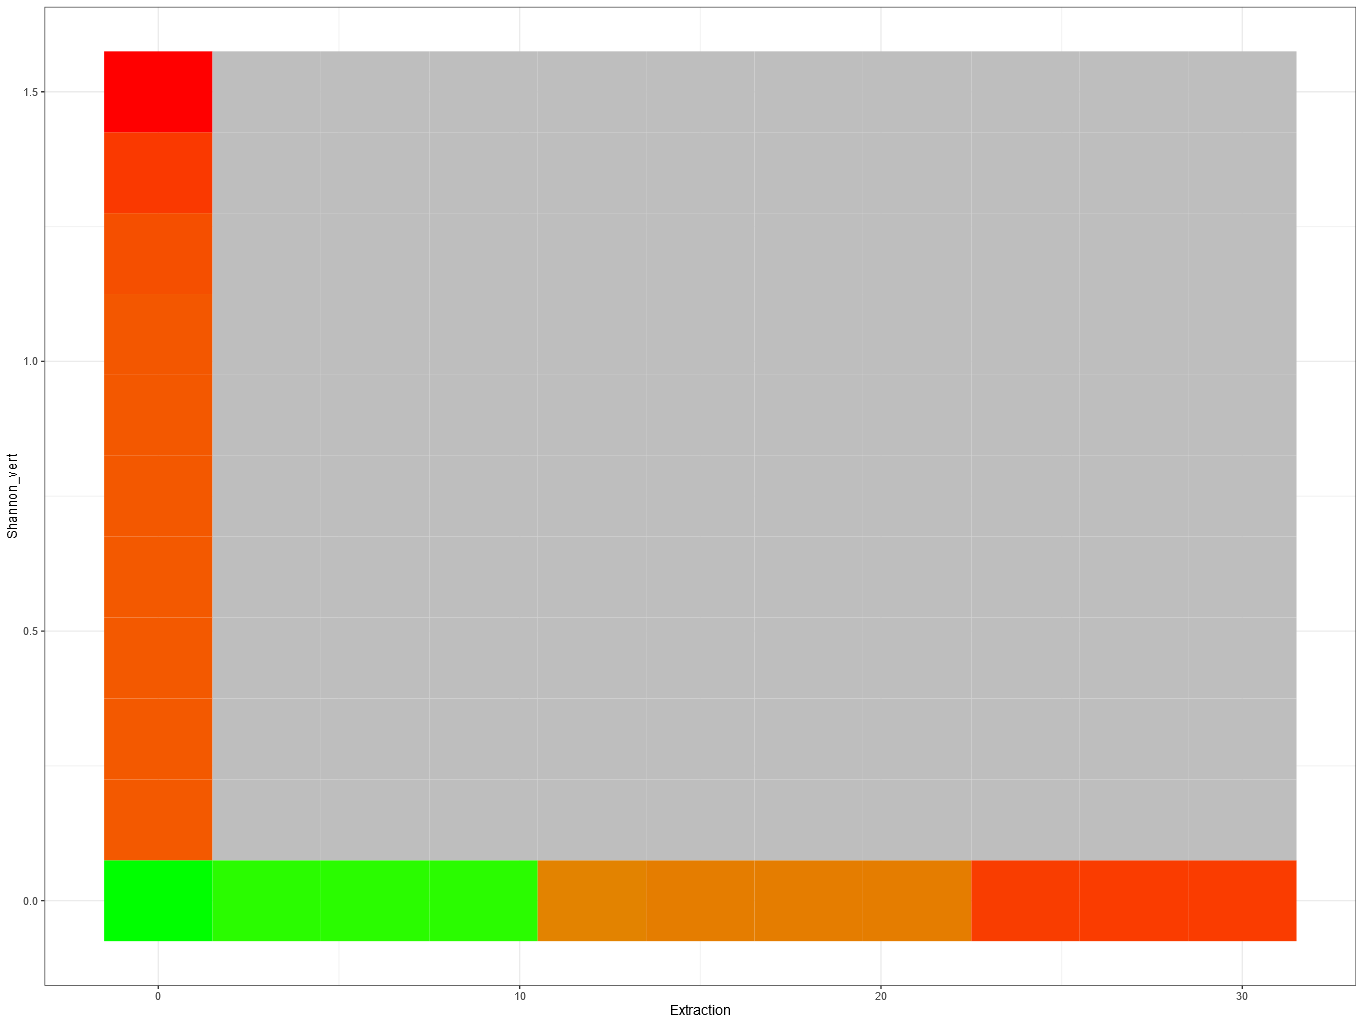
\includegraphics[width=\textwidth]{Figure/Sensi_ext_shvert.png}
%    \caption{Figure : Volume of viability kernel function of constraints}
%    \label{fig:sensi}
%\end{figure}

FOR NOW WASNT ABLE DO DO THE SENSI ANALYSIS (DO IT ON MONDAY IF I CAN OR NOT, NEED TO PRIORITIZE SOME STUFF)\\

Given the incompatibility of combining both constraints, where no trajectory can simultaneously adhere to our diversity criteria and extract 30 m³/ha of large wood every ten years, we opted for a separate analysis of the viability kernel for each set of constraints. This approach allows us to compare the results obtained under the distinct conditions and evaluate the trade-offs between maintaining diversity and meeting wood extraction requirements.

\subsection{Viable state with diversity or wood extraction constraints : Volume and visualization, what in common ?}

Volume of each viability kernel, which represents the number of states within the forest that can sustain either diversity or wood extraction constraints are shown in Table \ref{tab:Viability_kernel}. Notably, the volume of the viability kernel adhering to diversity constraints is 26,000 states, whereas the viability kernel for wood extraction constraints encompasses a significantly larger volume, consisting of 1.06 million states. This discrepancy shows that our diversity constraints impose more restrictions than wood extraction constraints. In practical terms, this means that, from the majority of states (98\%), the extraction of 30 m³/ha of large wood every ten years is permissible indefinitely, while only a minority of states (2\%) can maintain the more demanding diversity constraints. \\
To gain a nuanced understanding and characterize the forest states further, we projected them into the metric space (refer to Figure \ref{fig:Viability_kernel}). The choice of the metric space over the state space is driven by considerations of dimensionality (3 and 6, respectively) and the broader insights the metric space can provide regarding forest states, incorporating diversity metrics (Shannon index for species and vertical diversity) alongside basal area, as opposed to the mere count of stems in compartments. States within the viability kernel for wood extraction constraints (red points in \ref{fig:Viability_kernel}. A) exhibit a wide range of characteristics, these states can manifest almost any combination of features, except for a minimal necessary basal area. The key takeaway is that forests with the ability to sustain a specific wood extraction rate throughout the years can vary significantly in terms of species composition, vertical diversity, and basal area. Within the diversity viability kernel (blue and green points in \ref{fig:Viability_kernel}. B), states demonstrate more specific characteristics. This specificity is inherent, considering they must adhere to the constraints on diversity. But as they also need to sustain them over a ten-year period following a potential management intervention, certain diverse states are absent. Specifically, forests characterized by exceptionally high basal area, Shannon index, and vertical Shannon index (approximately 1, 1.5, and 400, respectively) are not included, even though they could potentially be viable for wood extraction (\ref{fig:Viability_kernel}. A). This observation suggests that densely packed forests with these particular characteristics might not be able to maintain their state within the diversity viability kernel over a 10-year management period, despite initially meeting the constraints.\\
The shared states (blue points in \ref{fig:Viability_kernel}. B) in both viability kernels indicate the potential for coexistence of biodiversity and sustainable wood extraction. However, the inability to determine trajectories with both constraints implies that forest conditions, initially supporting both, eventually become incompatible, necessitating a strategic choice in management practices to sustain either biodiversity or wood extraction.

\begin{table}[t!]
    \centering
    \begin{tabular}{l l l l l}
    \hline
    \hline
    \textbf{Constraints} & \textbf{State} & \textbf{Post control state} & \textbf{Control state} & \textbf{Association} \\
    \hline
    States studied & 1.12 M \\
    States in extraction viability kernel & 1.06M \\
    States in diversity viability kernel  & 26k \\
    States in both viability kernel & 17k \\
    \hline
    \hline
    \end{tabular}
    \caption{\underline{Number of states studied and in the different viability kernel}. Numbers are rouded and the states in both viability kernel represents the intersection between the two other ensemble.}
    \label{tab:Viability_kernel}
\end{table}

\begin{figure}[hb!]
    \centering
    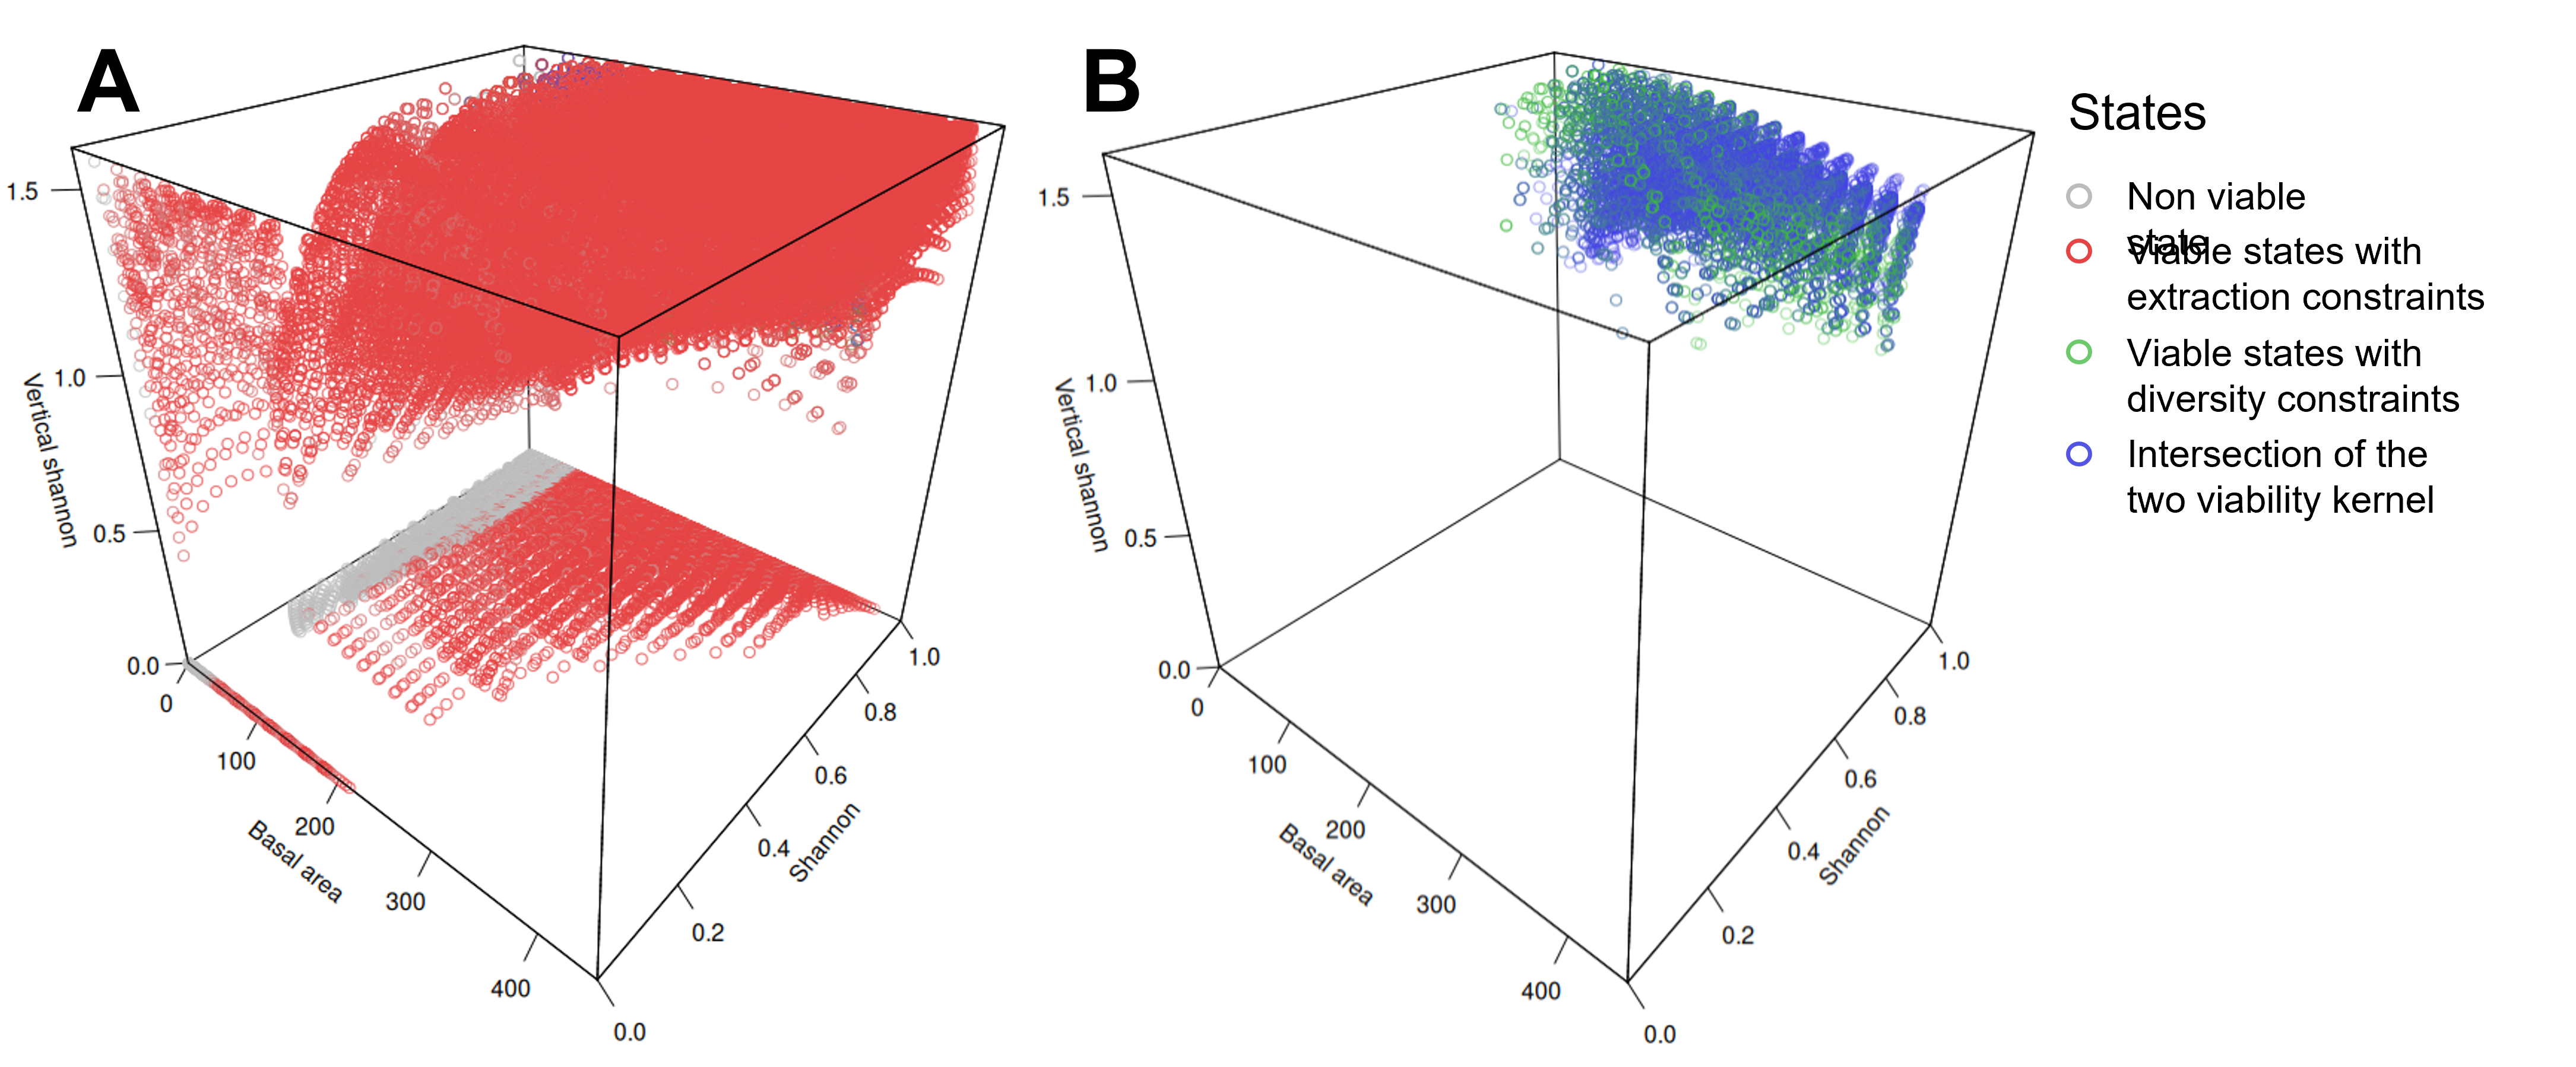
\includegraphics[width=\textwidth]{Figure/Results/Viability_kernel.png}
    \caption{\underline{Viability kernel in the metric space}. A : Representation of all states in the metric spaces, showing the viability kernel with wood extraction constraints (red) and the viability kernel with diversity constraints (green), the latter is shown alone in B for visibility. B : Representation of the viability kernel with diversity constraints, among them the states that are also in the viability kernel with wood extraction constraints are shown in blue. The number of states in each cathegory can be seen in detail in table \ref{tab:Viability_kernel}. Basal area is in m²/ha, Shannon index is dimensionless.}
    \label{fig:Viability_kernel}
\end{figure}

\subsection{Metric in the viability kernels}

J'AI RIEN FAIT POUR CA POUR L'INSTANT\\

\subsection{States in both Viability kernel and extraction constraints, critical states}

Exploring shared states might provide insights into the trade-off between diversity and wood extraction. Among them, some may possess common controls that are viable for both diversity and wood extraction, but the most interesting are those presenting none. This means that at this point, a choice is necessary between the two constraints and will imply different management trajectories. There are 7k of these critical states among the 17k in both viability kernels. These critical states lack shared controls, presenting scenarios where no common strategy exists (Figure \ref{fig:Criticals_states}).

The study of the respective control (number of stem cut for each species in the very large wood category) didn't show any clear pattern to discriminate between the two. The only notable caracteristic is that for diversity the number of stem for each species left in the very large wood category needs to be balanced, in order to keep the balance between the two species. However this kind of control can also be found in the wood extraction viability kernel. Then it is the specific combination of a state and a control that makes it critical. The only way to discriminate between the two is to look at the states that follows the control and the associated final state after ten years (Fig \ref{fig:Criticals_states}. B). States after a diversity trajectory exhibit lower basal area but to understand the different further and see how it can apply to a particular case, one critical state was chosen randomly and the associated trajectory studied (Fig \ref{fig:Extraction} and \ref{fig:Diversity}).

\begin{figure}[hb!] 
    \centering
    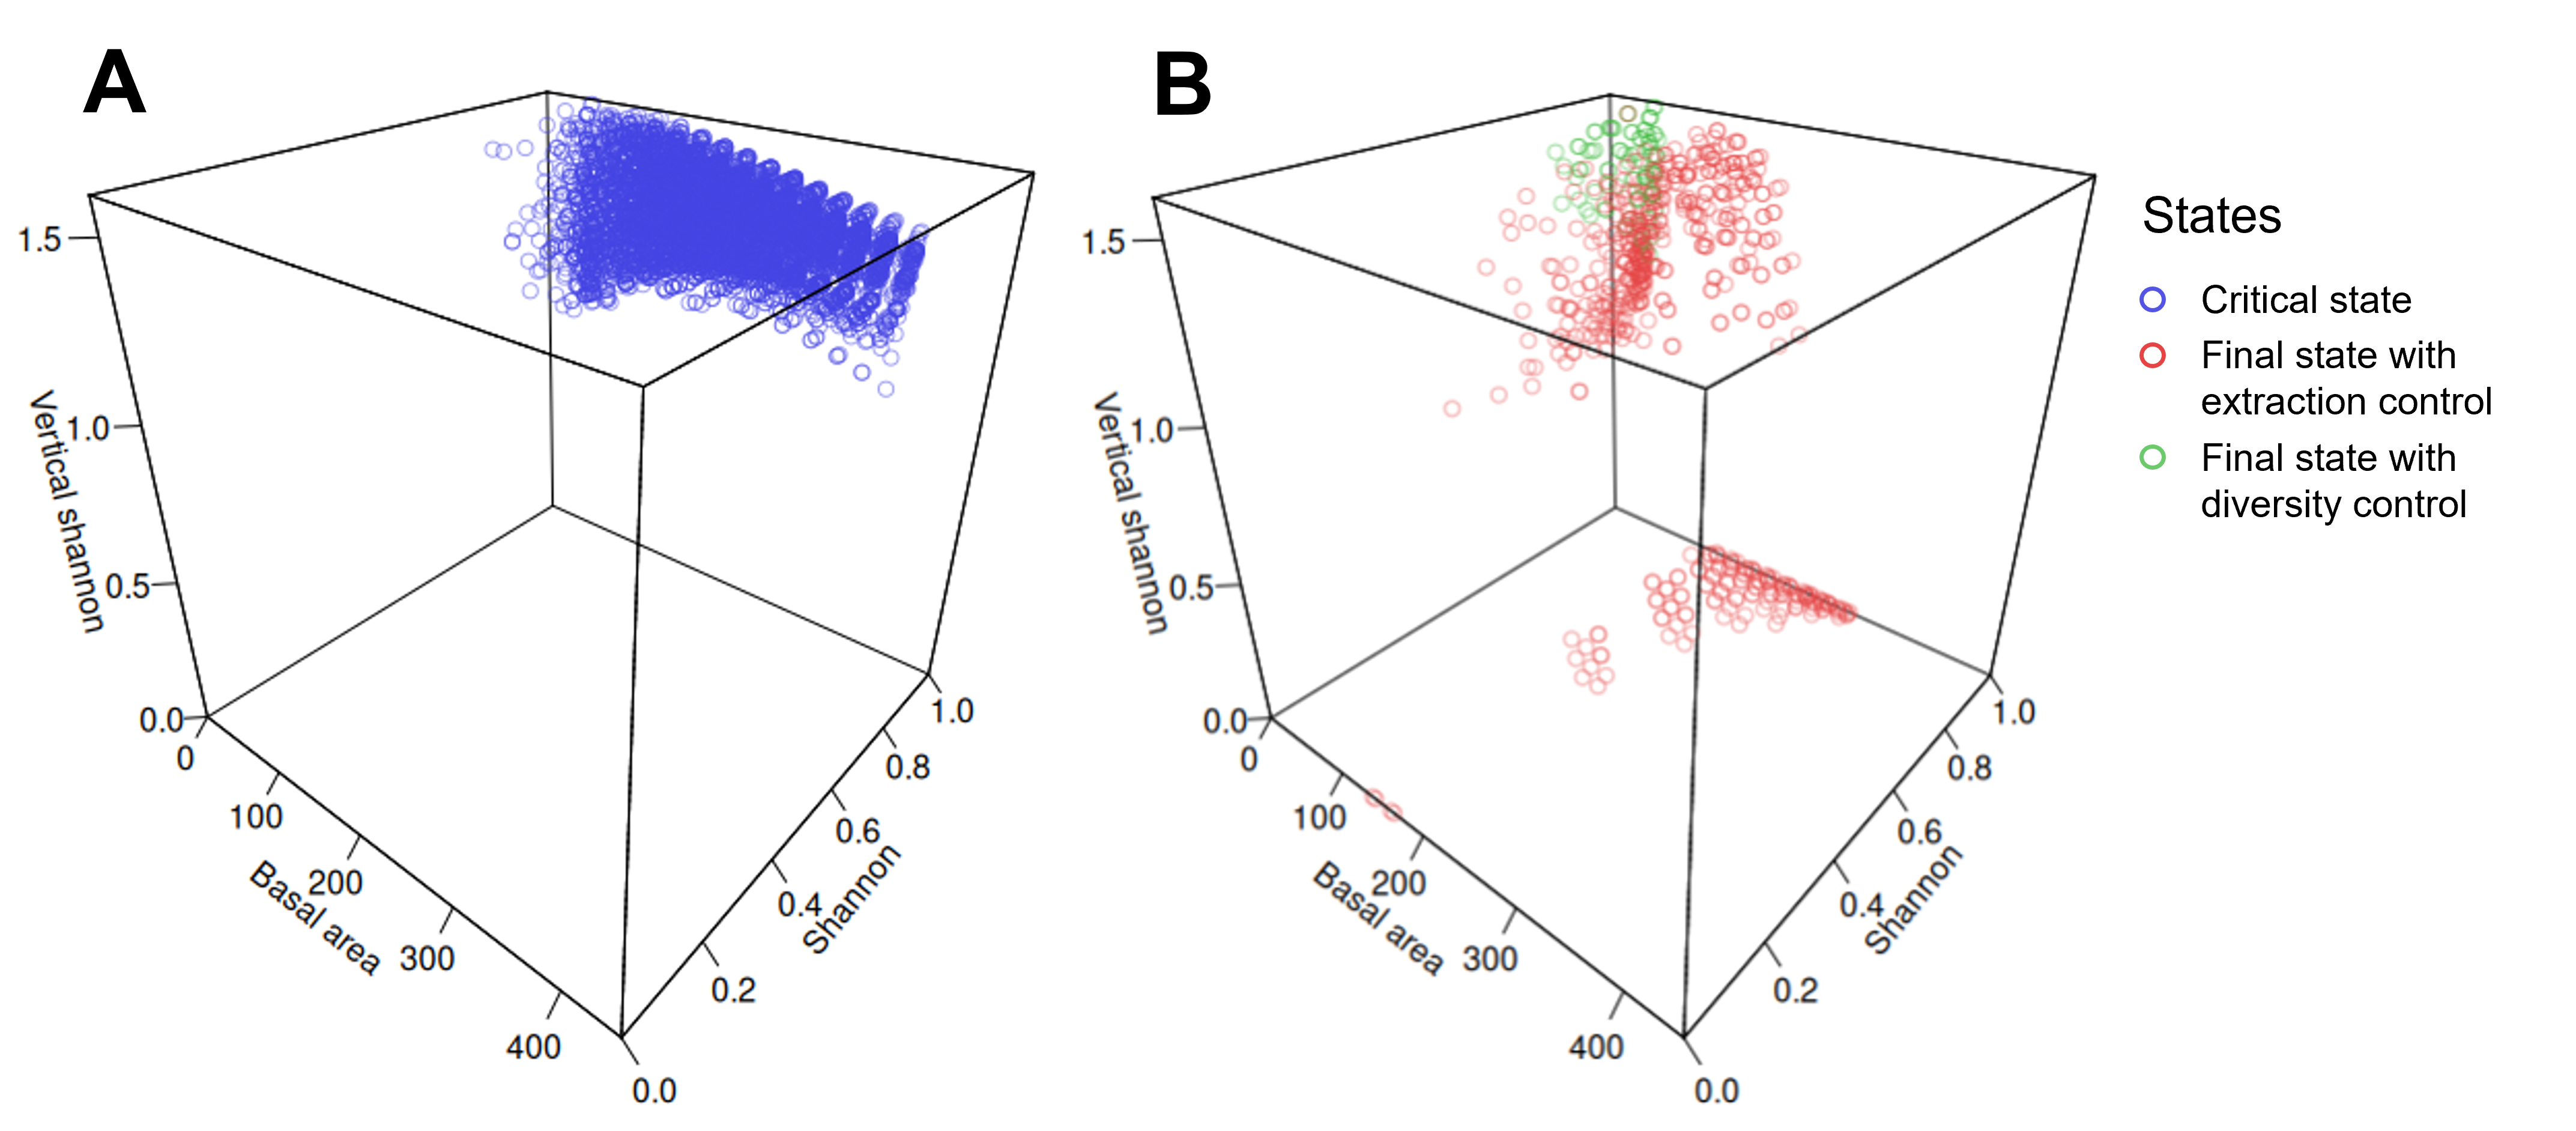
\includegraphics[width=\textwidth]{Figure/Results/Criticals_states.png}
    \caption{\underline{Critical states and final state divergence}. A : Representation of the critical states in the metric space. B : Representation of the states at t+10 after the choice of a diversity trajectory (green) or an extraction trajectory (red). Basal area is in m²/ha, Shannon index is dimensionless.}
    \label{fig:Criticals_states}
\end{figure}

\subsection{Study of one critical state and the following trajectory}

To analyze various trajectories from a critical state, we extracted trajectories from the viability kernel with wood extraction constraints (Fig. \ref{fig:Extraction}. A2) and from the viability kernel with diversity constraints (Fig. \ref{fig:Diversity}. A2). The controls extracted from these trajectories represent the number of stems left on the stand after the intervention. These controls were applied to the forest model, and the resulting forest dynamics are depicted in Figure \ref{fig:Extraction}. A1 and \ref{fig:Diversity}. A1.

An alternative approach would be to extract control as the number of stems removed from the stand (Fig. \ref{fig:Extraction2} and \ref{fig:Diversity2}). However, for technical reasons, using the control based on what stays on the stand allows us to stay closer to the dynamic of the model. This choice corrects the discrepancy between the model and the simulated dynamics introduced by the necessary discretization for viability analysis. Comparatively, using the control as the extracted stems deviates more from the model's dynamic. In fact, with the alternate choice (see appendix) of extracting what is cut, the trajectory is viable with the algorithm, but the model dynamic is not.

Opting for control based on what stays on the stand allows us to apply the resulting trajectory to the model dynamic, ensuring that our chosen metrics remain above our constraints (Fig. \ref{fig:Extraction}. B and \ref{fig:Diversity}. B). This is promising, indicating that the viability kernel serves as a solid approximation of the model's dynamic and can be leveraged to extract controls applicable to the model dynamic.

The incompatibility between extraction and diversity is evident, as the trajectory requiring diversity constraints involves no cutting, while the extraction trajectory necessitates cutting almost all trees in large wood layers (see Figure \ref{fig:Extraction} and \ref{fig:Diversity}), resulting in a stand with no vertical diversity.

Despite these promising aspects, imperfections are noticeable. The trajectory metric does not precisely match that of the model dynamic, and there is a gradual divergence of the trajectory from the model's dynamic over time, indicating instances where the model slowly deviates from a viable state present in the grid. It suggests that the viability may not be infinite.

\begin{figure}[b]
    \centering
    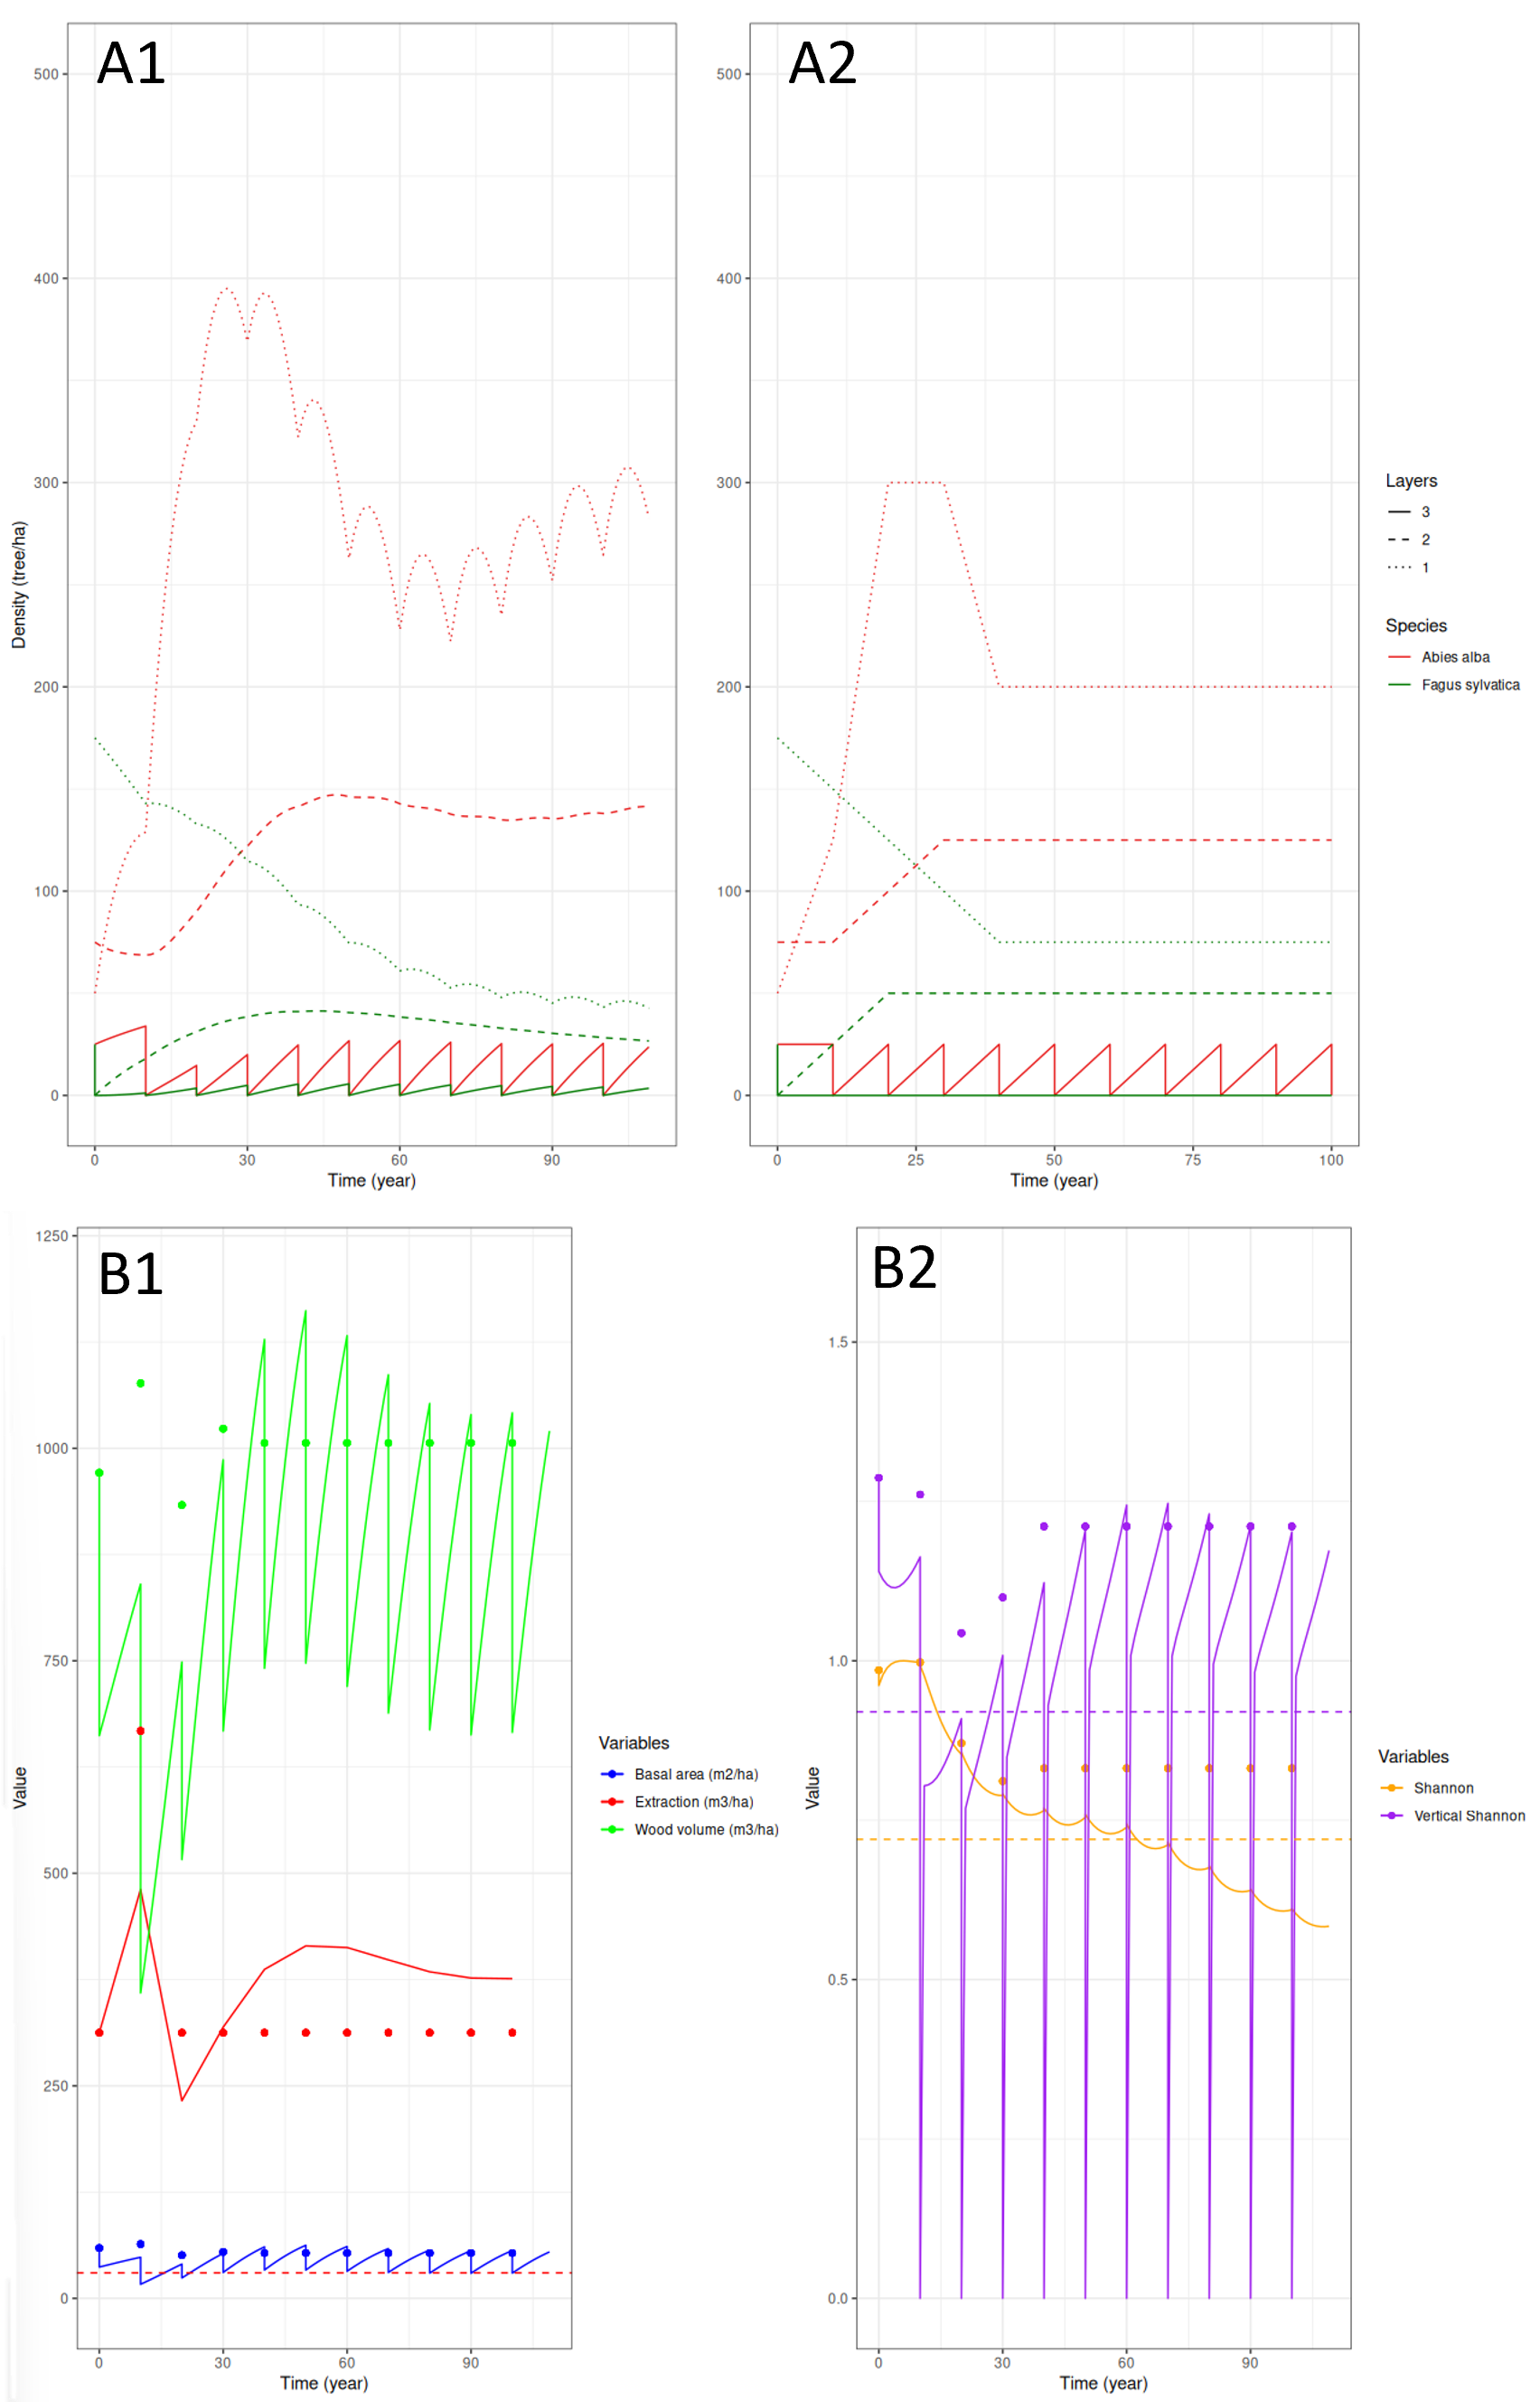
\includegraphics[height=0.8\textheight]{Figure/Results/Extraction.png}
    \caption{\underline{Trajectory of one critical state under wood extraction constraints and associated metrics}. Control where extracted from the viability kernel and applied to the model dynamic starting from the critical state (A1). On the left (A2) is the same dynamic but from the viability algorithm, meaning the dynamic is discretized into the grid. It is from this dynamic that the Control where extracted. B represents the metric evolution of this trajectory, for basal area, wood volume and extraction (B1) and for Shannon index and vertical Shannon index (B2). In these graphs the lines are te metric from our model dynamic (A1) and the points are the metric from the viability algorithm (A2). THe dotted lines represent the constraints that were set for the viability kernel.}
    \label{fig:Extraction}
\end{figure}

\begin{figure}[b]
    \centering
    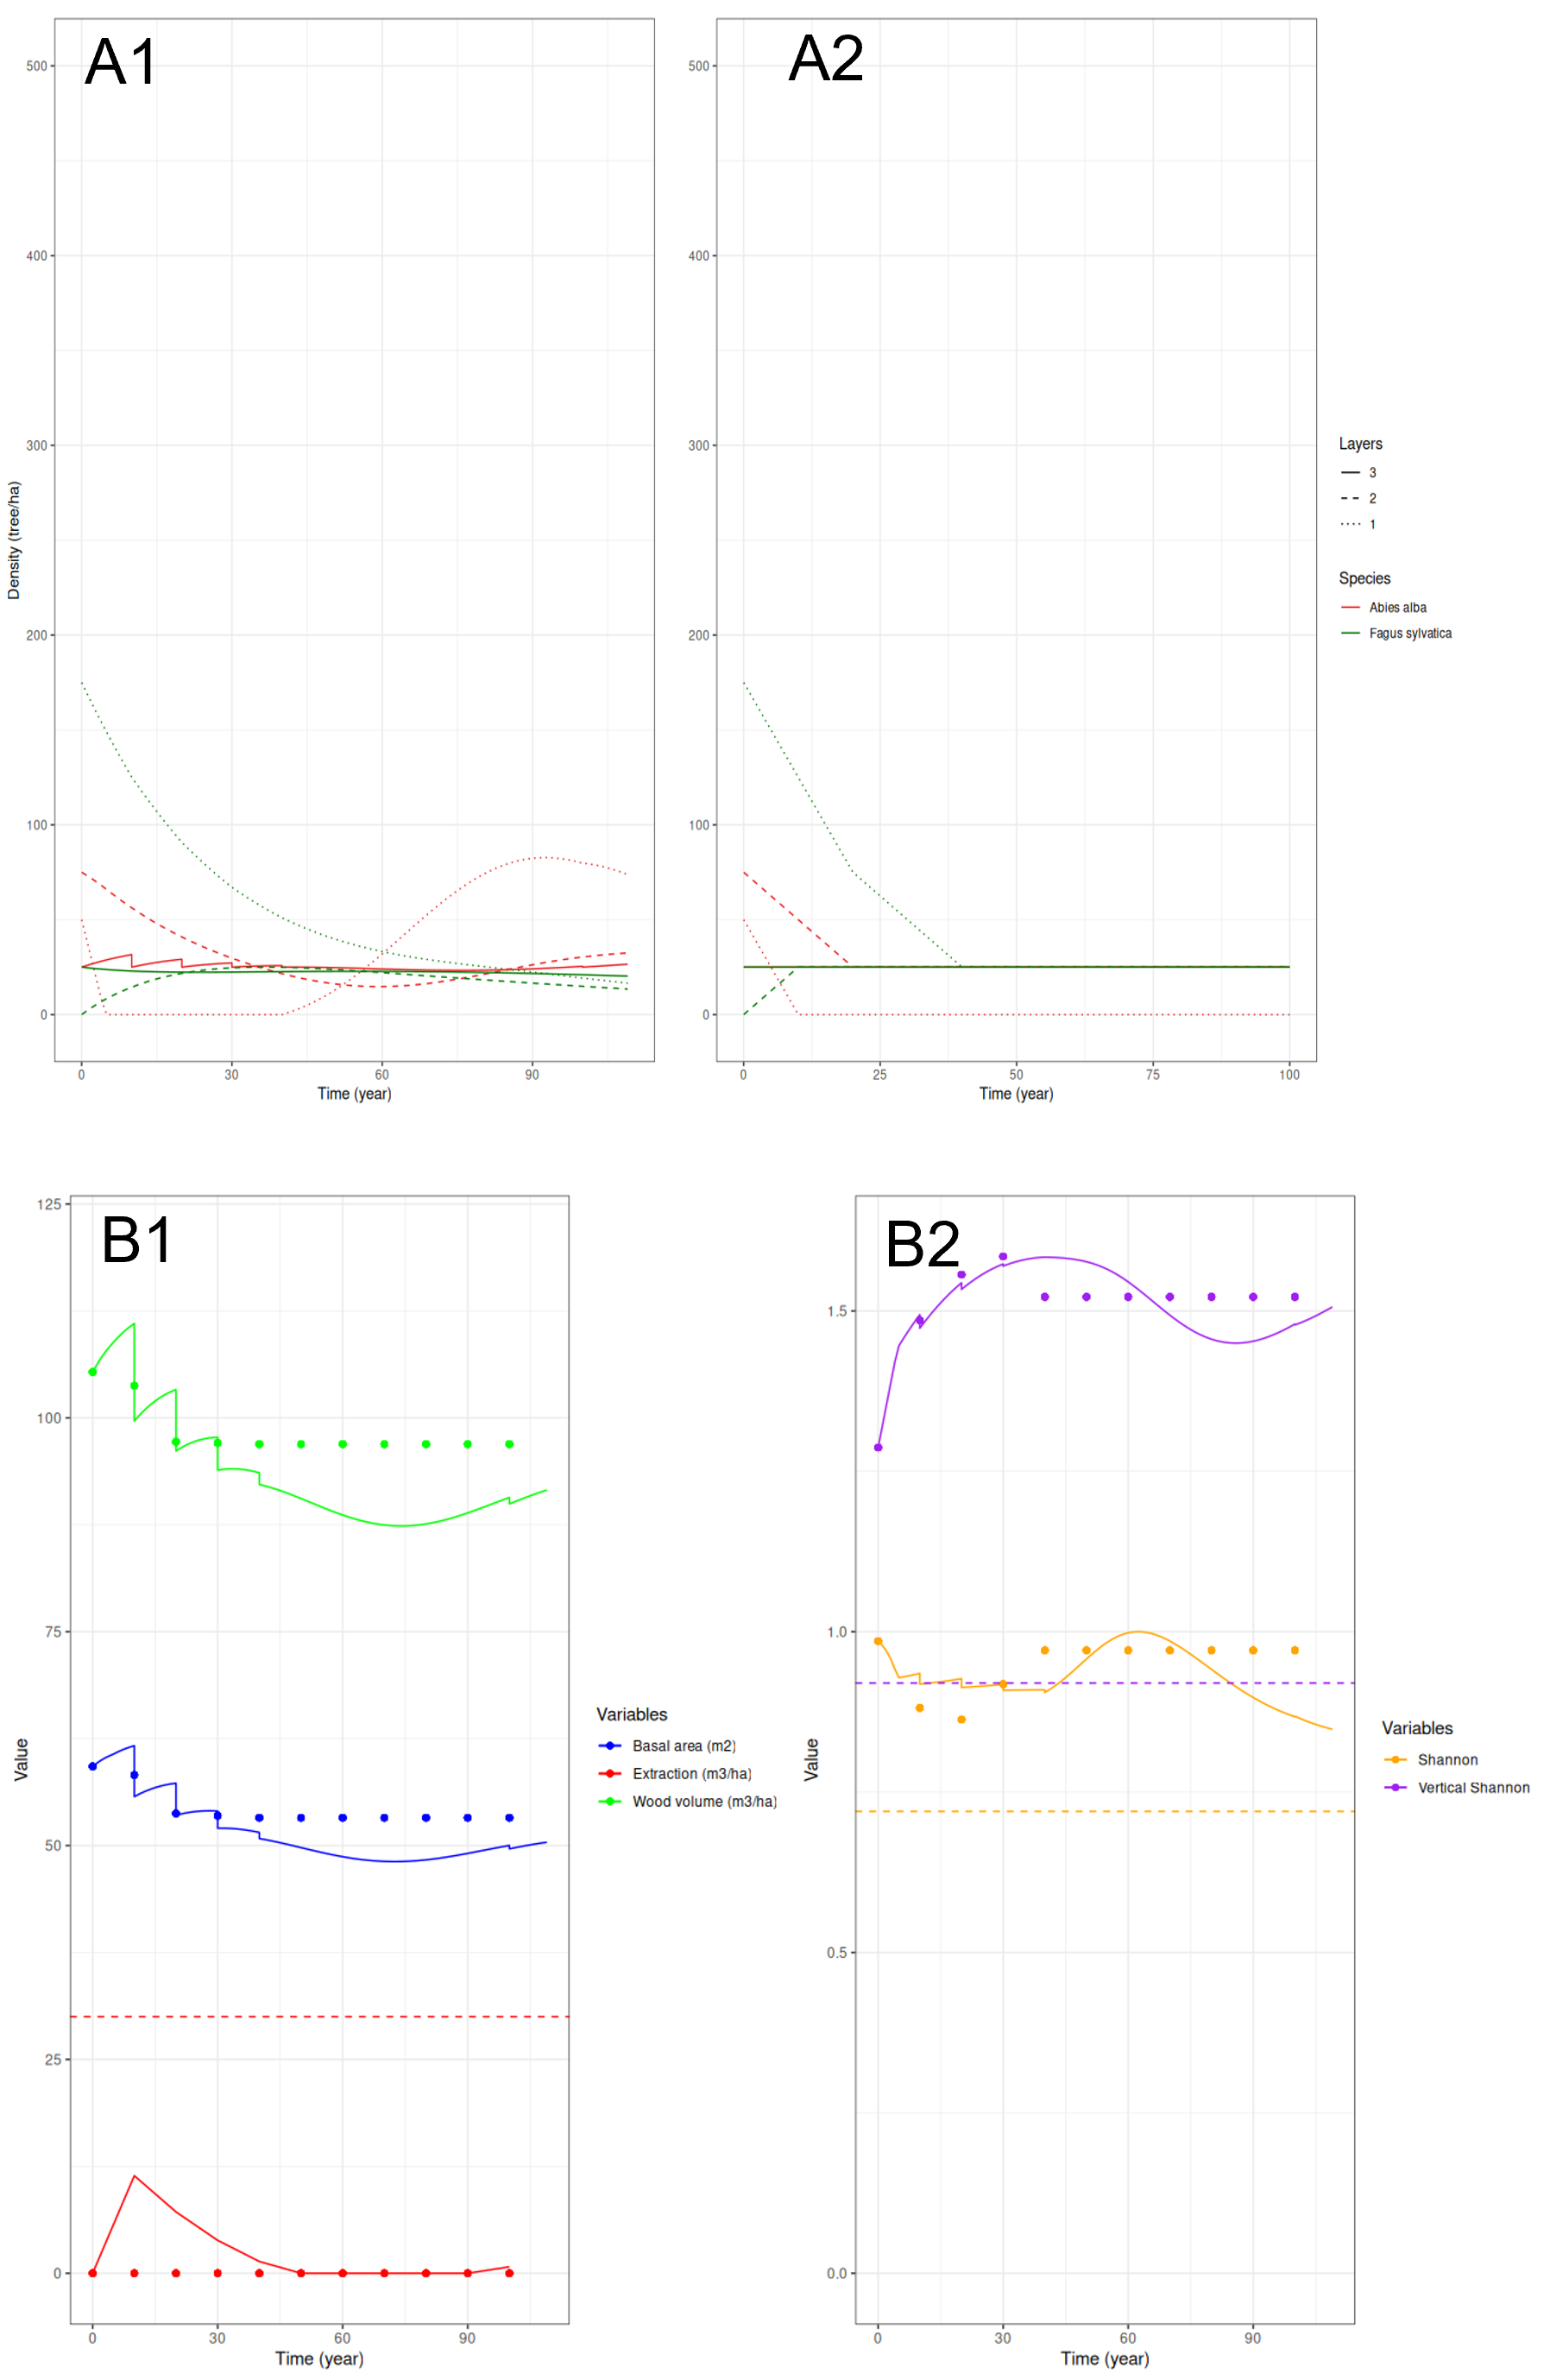
\includegraphics[height=0.9\textheight]{Figure/Results/Diversity.png}
    \caption{\underline{Trajectory of one critical state under diversity constraints}. See caption of Figure \ref{fig:Extraction} for details.}
    \label{fig:Diversity}
\end{figure}

\clearpage

\section{Discussion}

In order to be able to draw accurate conclusions from our results a few limits must be adressed. 

\textbf{Model}. The model we used is a very simplified representation of forest dynamics. It is based on a lot of assumptions and simplifications. A more  thorough parametrisation could have been achieved through data-driven approaches and sensitivity analyses on each parameter. Our parametrisation is based on a model (ForCEEPS) which himself is not a perfect representation of reality and posseses its own biases. A  more trustwothy model would allow to use more species in the following analyses. The inclusion of more species and layers would be essential to truly discuss diversity. Furthermore, the complexification of management practice is also necessary to encompasses all possiblilities; such as plantation practices, which directly address questions related to species choice and turnover in the face of climate change. The intricate dynamics of species selection become a crucial consideration, offering potential advantages in the context of forest plantation management ~\autocite{brockerhoffPlantationForestsBiodiversity2008}. Despite its limitations, the model serves as a good starting point, allowing us to highlight the technical challenges inherent in these analyses, including computational costs and grid size. The incorporation of state variables would necessitate improvements in hardware and algorithms, involving partitioning, GPU utilization, faster programming languages... ~\autocite{briasAcceleratingViabilityKernel2016}.

\textbf{Analyse discretisation}. The computational cost of our analyses limited the number of emulated forest states, leading to imperfect reproduction of our model dynamic by the studied grid. Consequently rajectories may differ and be viable in only one of the two cases. To validate our viability kernel approximation, a sensitivity analysis to grid size is crucial. This study could quantify the error arising from this approximation, providing insights into the trustworthiness of our results and aiding in achieving convergence~\autocite{saint-pierreApproximationViabilityKernel1994}.

\textbf{Constraints}. The constraints chosen for our model, focusing on diversity and wood extraction, are not exhaustive, as other ecosystem functions could have been considered. Understanding multifunctionality necessitates use of more diverse metric and further research on the links between those metrics and associated functions and services, allowing us to use them as proxies.

\textbf{Metrics}. The choice of metrics representing forest characteristics significantly impacts our conclusions. Sensitivity testing to validate the chosen metrics as proxies for species richness is crucial, as the conclusions drawn, whether related to composition or vertical diversity, hinge on these metrics ~\autocite{juckerClimateModulatesEffects2016, guldinRoleUnevenAgedSilviculture1996, noletComparingEffectsEven2018}. This complexity adds an additional layer of intricacy to understanding the connections between these metrics and the potential services forests could offer.

\textbf{Incompatibilities between diversity and wood extraction}. The first and main thing that our analyses revealed is the impossiblity of satisfying both objectives at the same time. As it doesn't seem to be impossible in reality (REF WHICH I DONT HAVE) it can be due to a number of things, the first one being the limit discussed above. In particular the vertical diversity on simply 3 layers plus the additional limitation of the harvating on the upper layer could lead to an incompatibility between wood extraction and vertical evenness. Another possibility is the control frequency, which could be too low for an adaptative management to be able to control the dynamic of the forest. Finally if some states show a compatibility at a certain time a quick overlook of multiple trajectories showed that a few stable states seem to attract the dynamic in each viability kernel and these are states where both constraints are not satisfied. These states can come from the discretisation of our system and may disapear with a finer grid. However it is also possible that they are real attractors of the dynamic and that the system is not viable in the long term with the kind of control applied here.

\textbf{Management}. A comparative analysis of Figure \ref{fig:Extraction}, \ref{fig:Diversity} and Figure \ref{fig:Extraction2}, \ref{fig:Diversity2} underscores the significance of defining and applying control to the dynamic. This choice—whether to focus on what is cut or what is left—not only poses technical challenges due to approximation but also prompts a shift in perspective. While potential corrections could arise through improved discretization, it also prompts broader reflections on how we interpret and utilize the outcomes of such analyses. Perhaps, concentrating on what we leave could be a more meaningful approach for finding  desirable dynamic, acknowledging that what remains is what shapes the trajectory of the subsequent dynamic.

\textbf{Conclusion and future work}. While there are avenues for refining and enhancing the precision of our results, as discussed earlier, our methods have unveiled promising insights. The ability to predict a sequence of interventions that can sustain a stand in a desirable state is a notable achievement. Further analyses could also be done from here, as the definition of dynamic adaptation pathway maps for more practical applications. Validation through the application of control trajectories to mechanistic models would provide crucial insights into the transferability of our conclusions. To advance this work, parallel improvement in the enrichment of the model, the exploration of additional metrics, and technical improvements (algorithms and hardware) is imperative, laying the foundation for future advancements in forest management strategies.

\clearpage

\begin{singlespace}
    \printbibliography
\end{singlespace}

\clearpage

% title page : Appendix

\begin{center}
    \textbf{\Large Appendix}
\end{center}

\pagenumbering{roman}

\renewcommand{\thefigure}{S.\arabic{figure}}
\setcounter{figure}{0}
% same for tables
\renewcommand{\thetable}{S.\arabic{table}}
\setcounter{table}{0}

\appendix

\section{Kohyama model parametrisation}

We are starting with a 3 layers 3 species system with a mixture of possible species : \textit{Abies alba}, \textit{Betula pendula}, \textit{Fagus sylvatica}, \textit{Picea abies}, \textit{Pinus sylvestris}, \textit{Quercus pubescens}. The layers are defined by dbh (cm) interval : [0,22.5], [22.5,67.5], [67.5+[. We have to define all parameters in Table \ref{tab:coeftoparam}.

\begin{table}[H]
    \centering
    \begin{tabular}{l l l}
    \hline
    \hline
    \multicolumn{3}{l}{\textbf{By species}, $sp$} \\
    \hline
    $b_{sp,1}$     & optimal birth probability                              & $ha^{-1}.year^{-1}$ \\
    $Cb_{sp,1}$    & birth susceptibility to superior foliage density       & $ha.m^{-2}$       \\
    $m_{sp}$       & probability of intrinsic mortality                     & $year^{-1}$ \\
    $Cg_{sp}$      & growth susceptibility to superior foliage density      & $ha.m^{-2}$           \\
    $Cm_{sp}$      & mortality susceptibility to superior foliage density   & $ha.m^{-2}$           \\    
    \\
    \multicolumn{3}{l}{\textbf{By layer $l$}} \\
    \hline
    $\phi_{l}$  & mean basal area per tree in layer $l$        & $m^{2}.ha^{-1}$  \\
    \\
    \multicolumn{3}{l}{\textbf{By species $sp$ and layer $l$}} \\
    \hline
    $g_{sp,l}$     & optimal probability of transition from layer $l$ to the next & $.year^{-1}$ \\
    \\
    \hline
    \hline
    \end{tabular}
    \caption{Parameters that we have to define numerically}
    \label{tab:coeftoparam} 
\end{table}

\subsection{Parameters deduced form litterature of ForCEEPS and ForClim}

\subsubsection{Basal area}

Basal area is defined as the area of the cross subsection of the tree at breast height (1.3m). It is a good indicator of the density of the forest. It is defined as : 

\begin{equation}
    \phi_{l} = \frac{\pi}{4} * \overline{D_{l}}^2
\end{equation}

With $\overline{D_{l}}$ the mean diameter in layer $l$. (i.e. 11.25, 45, 100 cm).\\

\subsubsection{Intrinsec Mortality}

Mortality was defined axactly as in ForCEEPS, as the inverse of the life expectancy of the species ($A_{max}$) multiplied by a factor $c_{mort}$ = 4.605.
\begin{equation}
    m_s = \frac{c_{mort}}{A_{max_s}}
\end{equation}

$A_max$ can be found in the thesis on ForClim ~\autocite{bugmannEcologyMountainousForests1965} or the supplementary data of ForCEEPS ~\autocite{morinForestSuccessionGap2021}

\subsubsection{Optimal Growth}

Optimal growth is defined in ForCEEPS ~\autocite{morinForestSuccessionGap2021} as :

\begin{equation}
    \Delta D_{\mathrm{opt}_i}(t+1)=g_s \frac{D_i(t)\left(1-\frac{H_i(t)}{H_{\max _s}}\right)}{2 H_{\max _s}-b_{\max _s} \times \exp \left(\left(\frac{-s_s}{b_{\max _s}} D_i(t)\right) \times\left(\frac{-s_s}{b_{\max _s}} D_i(t)+2\right)\right.}
\end{equation}

With $g_s$ the growth rate, $D_i$ the diameter of the tree, $H_i$ the height of the tree, $H_{\max _s}$ the maximum height of the species, $b_{\max _s}$ the maximum heigth of the species above breast ($b_{\max _s} =  H_{\max _s} - 1.37$), and $s_s$ the shape parameter of the species. $g_s$, $H_{\max _s}$, and $s_s$ can be found in the appendix ~\autocite{morinForestSuccessionGap2021}. $H_i$ is also defined as a function of $D_i$ :

\begin{equation}
    H_i(t)=b+b_{\max _s}\left(1-\exp \left(-\frac{s_s}{b_{\max _s}} D_i(t)\right)\right)
    \label{eq:height}
\end{equation}

This gives a function $f(D_i) = \Delta D_{\mathrm{opt}_i}(t+1)$, which is the growth of the tree as a function of its diameter.

\begin{figure}
    \centering
    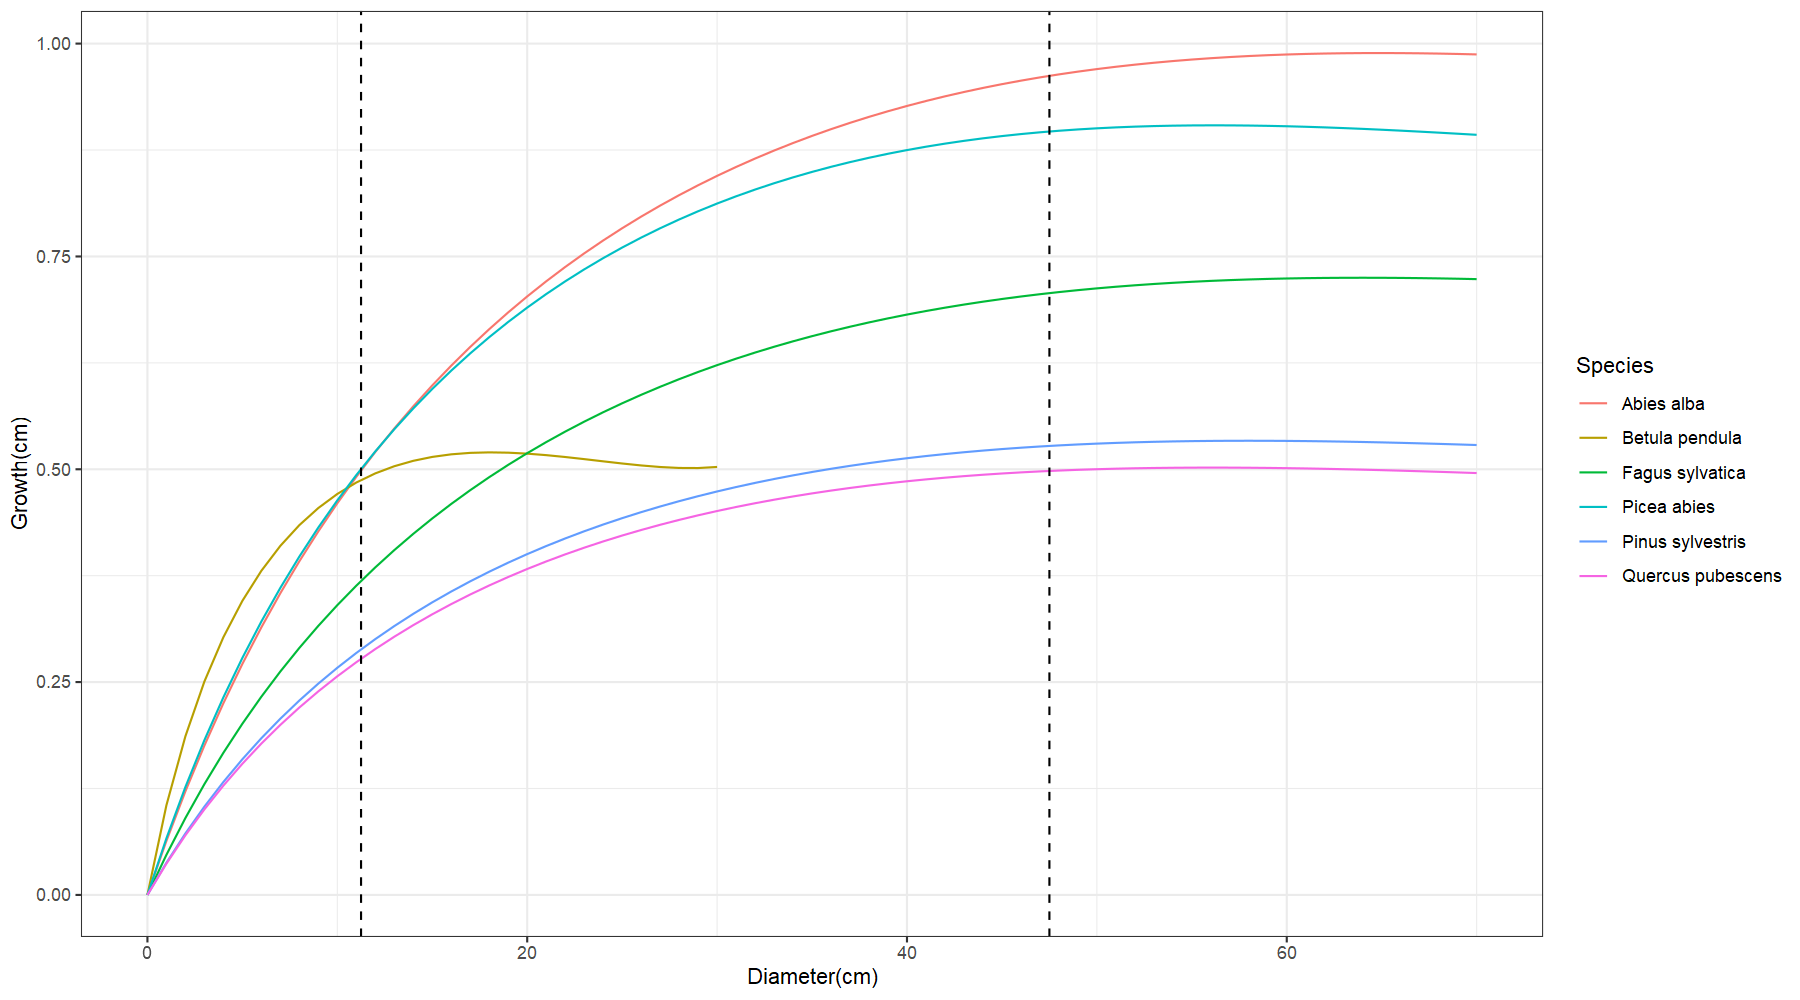
\includegraphics[width=\textwidth]{Figure/Parametrisation/Growth_diameter.png}
    \caption{Growth as a function of diameter for the 5 species}
    \label{fig:growth_diameter}
\end{figure}

As our model does not account for a change of growth with diameter we took the growth from the mean diameter of our two interval : [0, 22.5] and [22.5, 67.5] (i.e. 11.25 and 45). It gives :

\begin{table}[H]
\begin{center}
    \begin{tabular}{lll}
    \hline
    Species & Growth 1 & Growth 2 \\ \hline
    \textit{Abies alba} & 0.5 & 0.96 \\
    \textit{Betula pendula} & 0.5 & 0 \\
    \textit{Fagus sylvatica} & 0.37 & 0.71 \\
    \textit{Picea abies} & 0.5 & 0.9 \\
    \textit{Pinus sylvestris} & 0.29 & 0.53 \\
    \textit{Quercus pubescens} & 0.28 & 0.5 \\ \hline
    \end{tabular}
    \caption{Growth for the 5 species and two below layers}
\end{center}
\end{table}

Growth is the number of cm added to the diameter of the tree each year. To get the transition probability to the next layer with the assumption that tree dbh are uniformly distributed in each layer we need to divide this value by the diameter difference of the layer (See Tab. \ref{tab:final_param}).

\subsubsection{Optimal Esthablishment}

Establishment is a process that is still not well understood. In ForCEEPS optimal establishment (if all the threshold for establishment are met) is the same for every species : 0.006 individu/m2/year. We will use this value for our model for every species.

\subsubsection {Light competition}

Proportionality between the species is known (see ForClim Ly (growth) and La(birth)), as mortality due to light competition is due to the absence of growth we used the same proportionality between species.

\begin{table}[H]
\begin{center}
    \begin{tabular}{lll}
    \hline
    Species & Ly (growth, mortality) & La (birth) \\ \hline
    \textit{Abies alba} & 0.05 & 1 \\
    \textit{Betula pendula} & 0.3 & 9 \\
    \textit{Fagus sylvatica} & 0.05 & 1 \\
    \textit{Picea abies} & 0.1 & 5 \\
    \textit{Pinus sylvestris} & 0.3 & 9 \\
    \textit{Quercus pubescens} & 0.3 & 7 \\ \hline
    \end{tabular}
    \caption{Sensitivity for light competition}
    \label{tab:prop_sensitivity}
\end{center}
\end{table}

If we have a relative sensitivy of our species to light availability we still have to get the global coefficient linked to this sensitivity for growth, birth and mortality. We cannot extract the parameters from a simplification as we used a negative linear function, which is not the case in ForCEEPS. We will use the data from ForCEEPS to fit our parameters.

\subsection{ForCEEPS input data and results}

ForCEEPS simulations where used to adjust the dynamic of the system. 6 species where chosen to do so : \textit{Abies alba}, \textit{Betula pendula}, \textit{Fagus sylvatica}, \textit{Picea abies}, \textit{Pinus sylvestris}. We chose a constant climate for 300 years drawn randomly from meteorologic data from Bern between 1950 and 2000 (resulting climate can be found in Fig. \ref{fig:climate}). We used the same initial forest structure for all simulations : 10 trees per species per layer. We did 20 simulations of 1000m2 patch for each species association. We then took the mean of the 20 simulations and multiplied it by 10 to get the number of trees per hectare. We then fitted the parameters of the model to get the same dynamic as the ForCEEPS simulations.

\subsubsection{Climate}

Climate was taken randomly for each months in the climate data from 1950 to 2000 (Bern), to get a constant climate. To be sure to have non limiting precipitation they were all multiplied bya factor 10.

\begin{figure}[H]
    \centering
    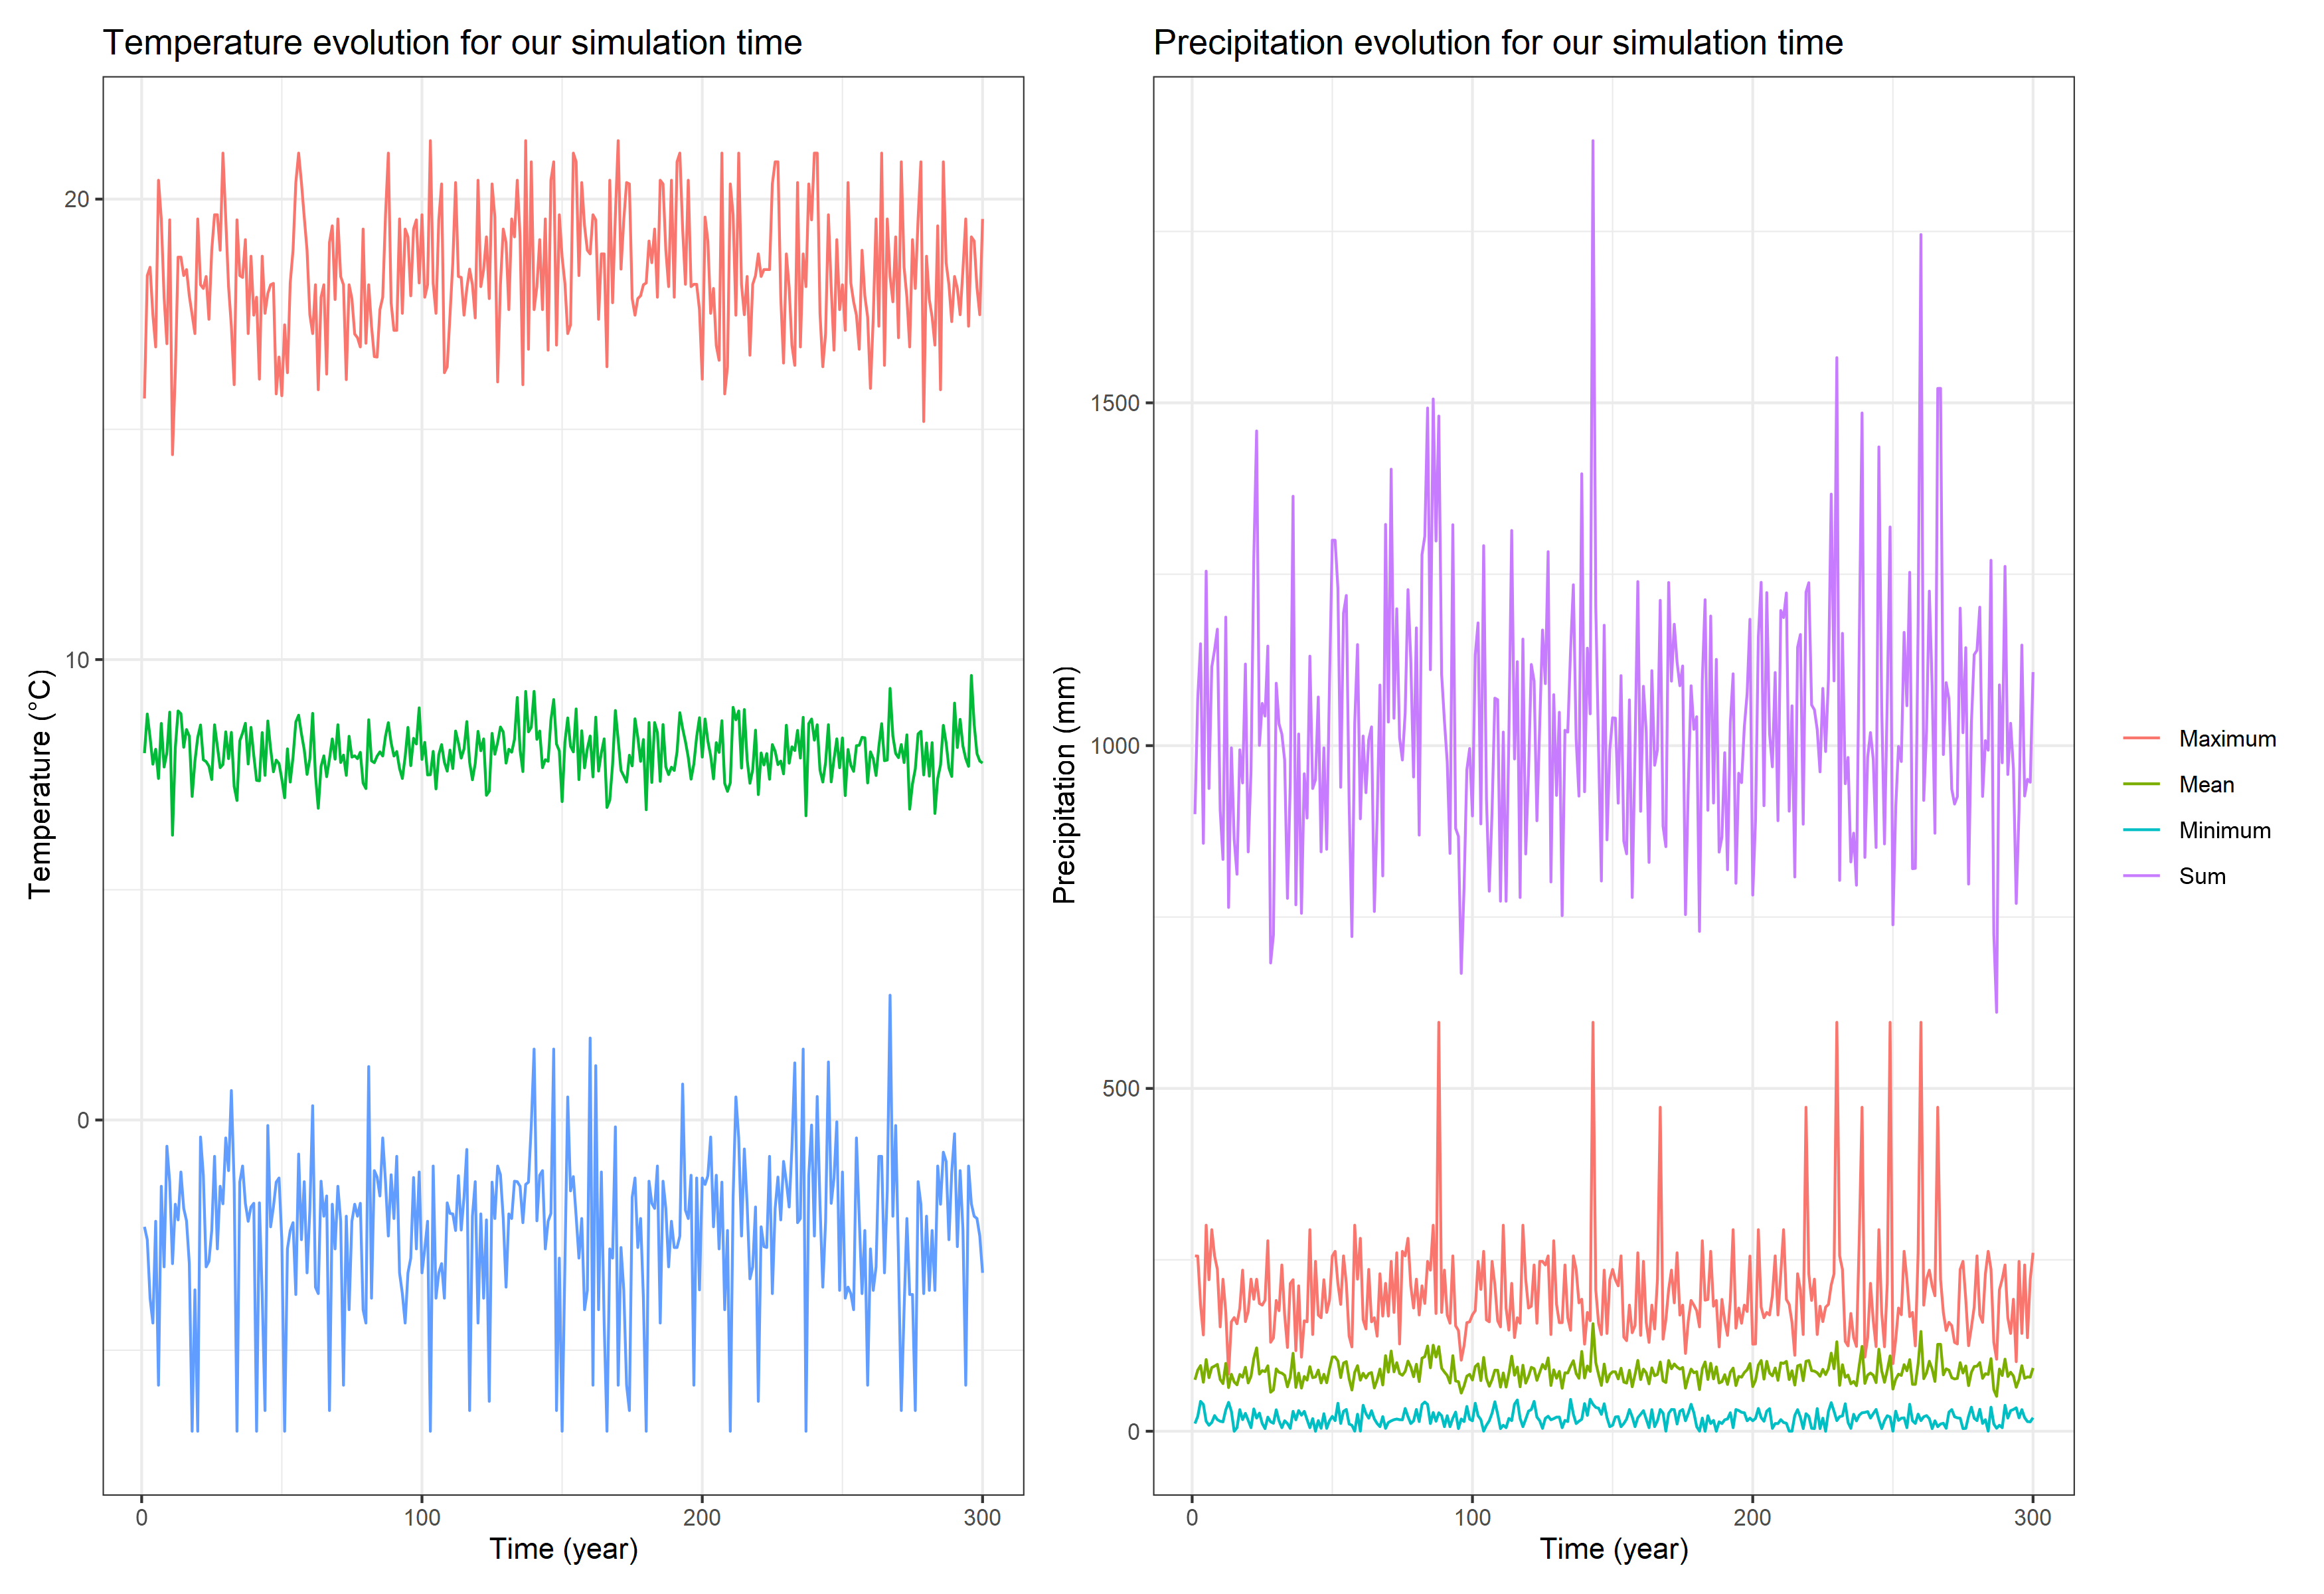
\includegraphics[width=1\textwidth]{Figure/Parametrisation/Climate_simul.png}
    \caption{Climate for our ForCEEPS simulation}
    \label{fig:climate}
\end{figure}

\subsubsection{setup parameters}

For the setup parameters we used non limiting values for water and nitrogen. The parameters can be found in the github documents (file Basic.setup), and are the same for all simulations.

Result of the simulation are in color in Fig. \ref{fig:Simulation_fit}.

\subsubsection{Fitting the parameters}

To fit the parameter we used the function optim in R with the following parameters :

\begin{tcolorbox}
result <- optimParallel(start point, function to minimize, lower = rep(0,3), upper = rep(0.1,3), method = ''L-BFGS-B'')
\end{tcolorbox}

Method "L-BFGS-B" (see optim documentation ~\url{https://www.rdocumentation.org/packages/stats/versions/3.6.2/topics/optim}) allows box constraints, that is each variable can be given a lower and/or upper bound. The initial value must satisfy the constraints. This uses a limited-memory modification of the BFGS quasi-Newton method.  "BFGS" is a quasi-Newton method (also known as a variable metric algorithm), specifically that published simultaneously in 1970 by Broyden, Fletcher, Goldfarb and Shanno. This uses function values and gradients to build up a picture of the surface to be optimized.

I only fit three non specific parameters LCg (light competition for growth), LCm (light competition for mortality) and LCb (light competition for birth). In the model they are then multiplied by the sensitivity of the species to light competition (see Tab. \ref{tab:prop_sensitivity}).

\subsubsection{Results}

% figure sur toute une page dans le sens de la longueur (landscape)
\begin{sidewaysfigure}[ht]
    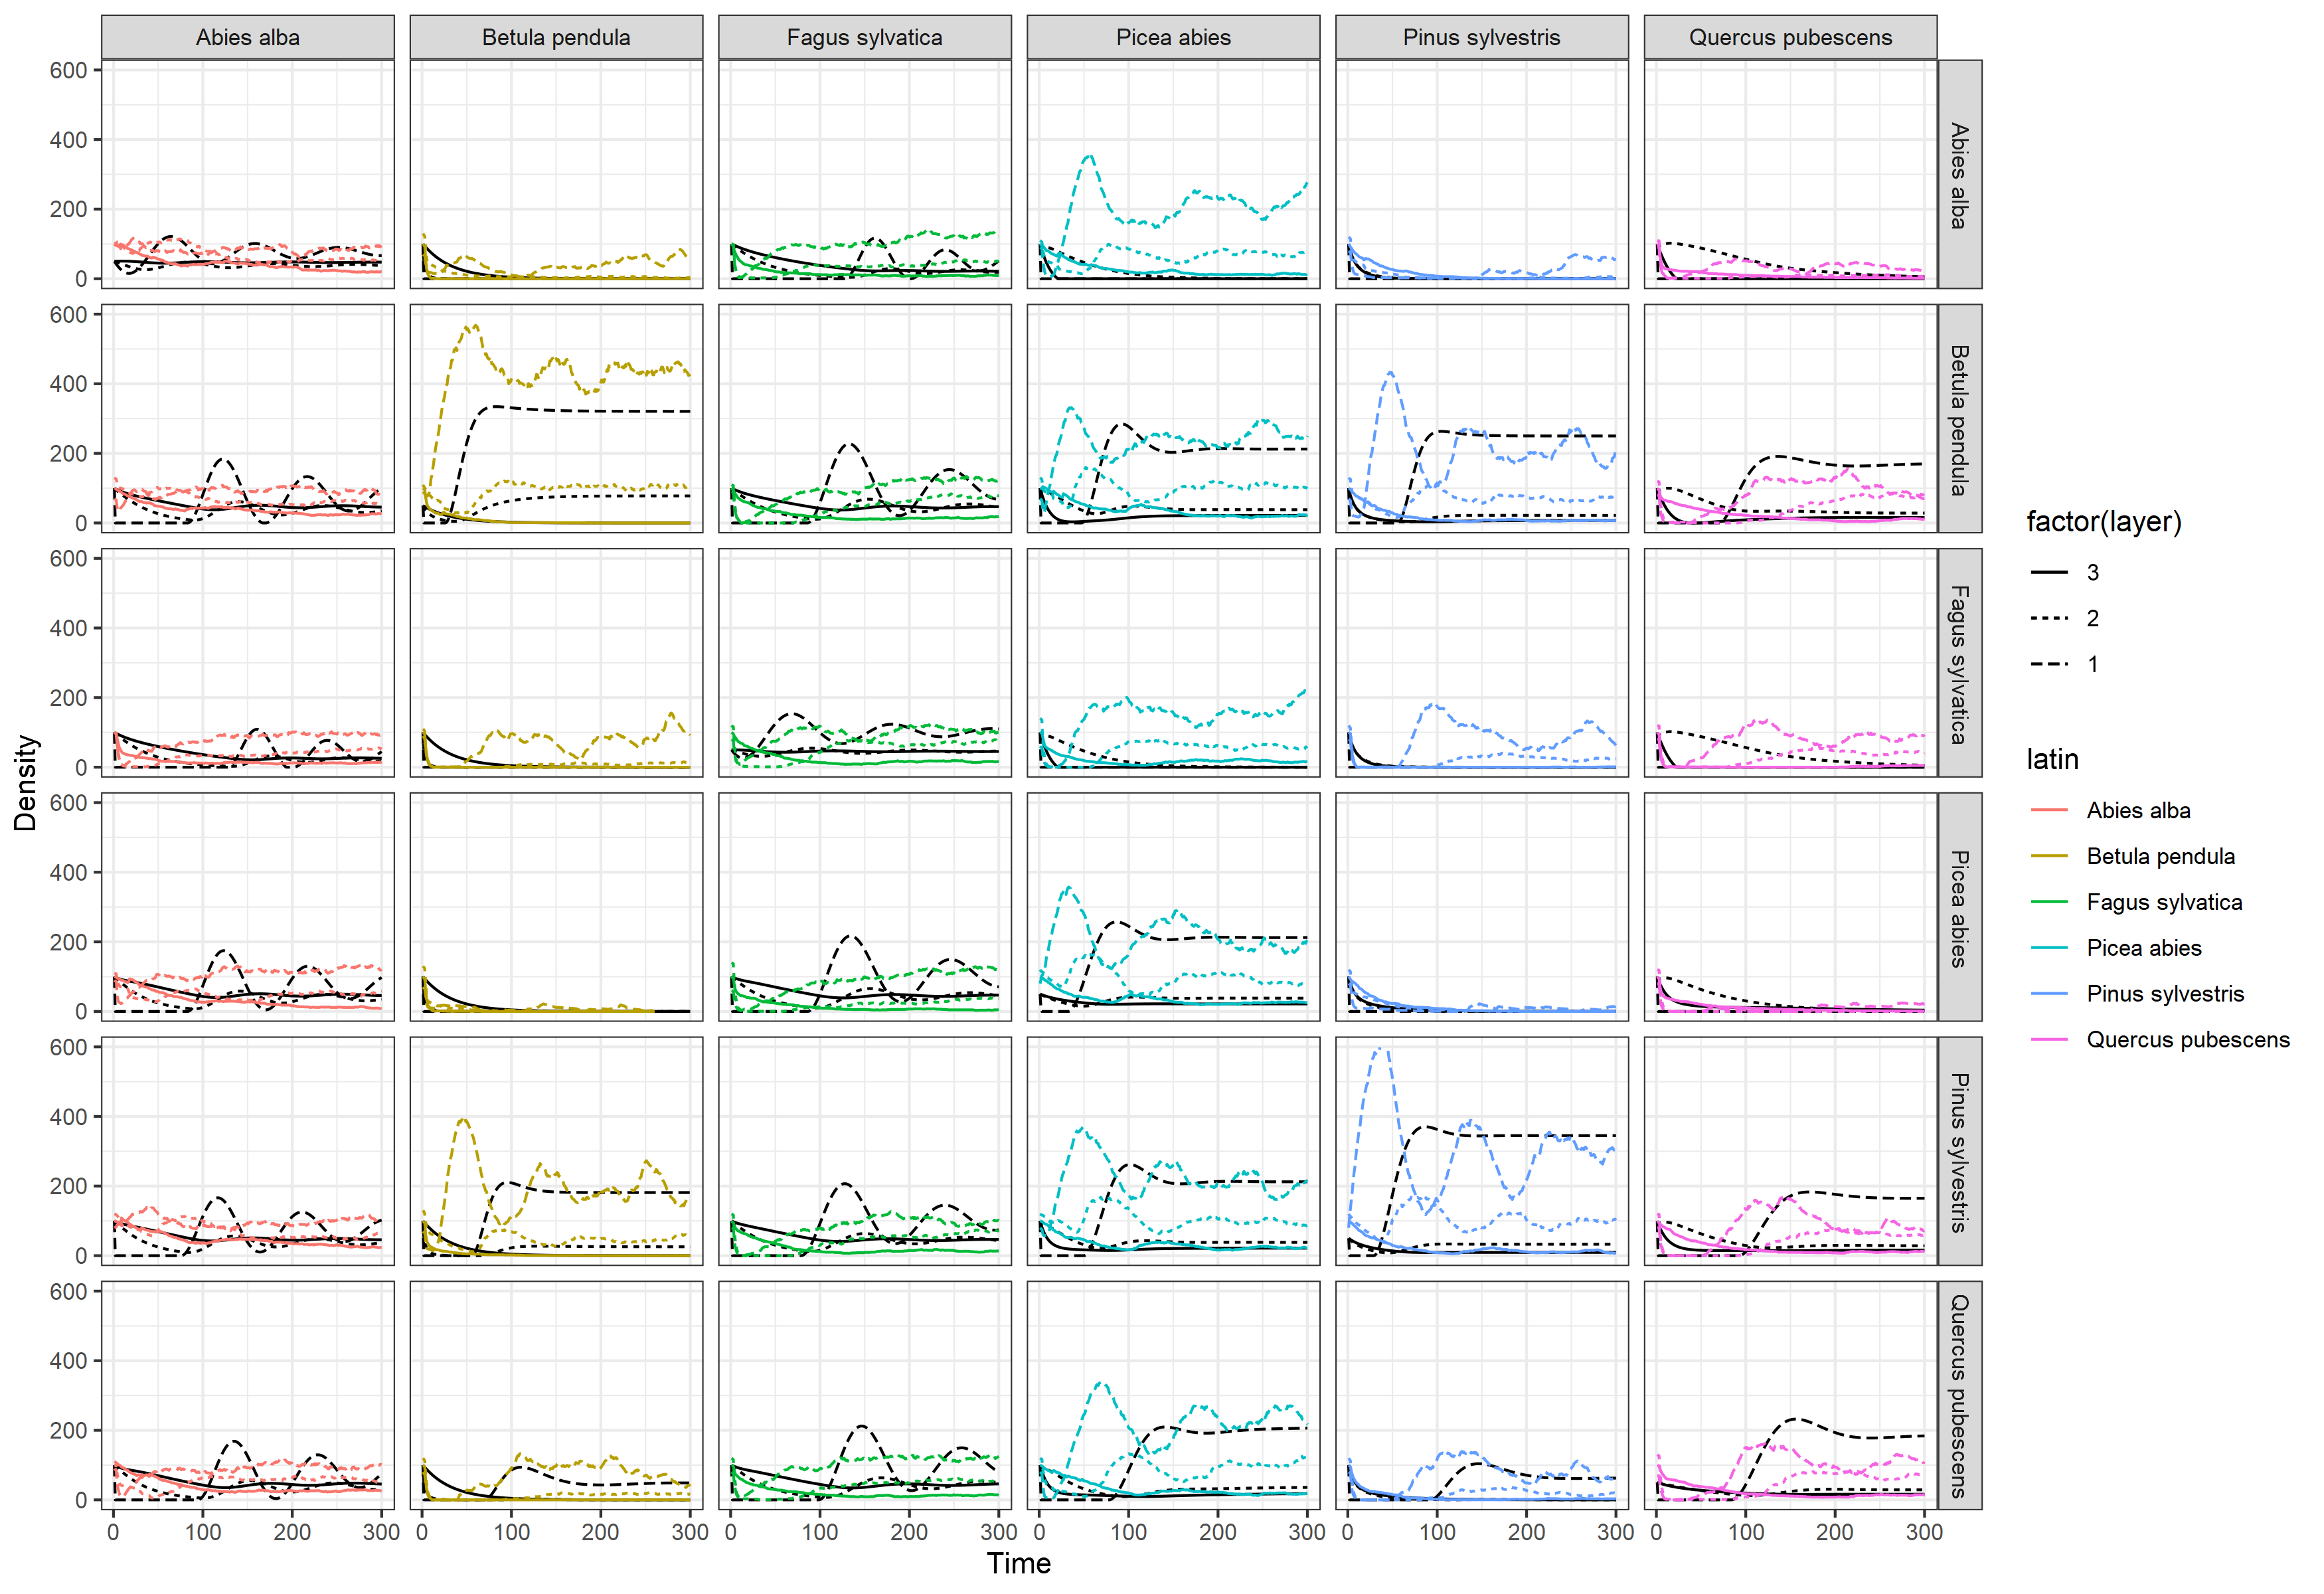
\includegraphics[width=\textwidth]{Figure/Parametrisation/Simulation_fit.png}
    \caption{Fit Kohyama model (color) on ForCEEPS simulation (black) for individual species}
    \label{fig:Simulation_fit}
\end{sidewaysfigure}

\begin{table}[H]
\begin{center}
    \begin{tabular}{llllllll}
    \hline
    Species & b (/ha/an) & m (/year) & g1 (/year) & g2 (/year) & LCb & LCm & LCg \\ \hline
    \textit{Abies alba}       & 60 & 0.013 & 0.022 & 0.021 & 0.0059 & 0.0046 & 0.0059 \\
    \textit{Betula pendula}   & 60 & 0.031 & 0.022 & 0     & 0.0295 & 0.0229 & 0.0295 \\
    \textit{Fagus sylvatica}  & 60 & 0.012 & 0.016 & 0.016 & 0.0531 & 0.0413 & 0.0531 \\
    \textit{Picea abies}      & 60 & 0.015 & 0.022 & 0.02  & 0.0531 & 0.0413 & 0.0531 \\
    \textit{Pinus sylvestris} & 60 & 0.023 & 0.013 & 0.012 & 0.0059 & 0.0046 & 0.0059 \\
    \textit{Quercus pubescens}& 60 & 0.008 & 0.012 & 0.011 & 0.0413 & 0.0321 & 0.0413 \\ \hline
    \end{tabular}
    \caption{Parameters found for the 5 species}
    \label{tab:Final_param}
\end{center}
\end{table}

\subsection{Volume allometry}

Volume was calculated with the formula from ~\autocite{deleuzeEstimerVolumeTotal2014} :

\begin{equation}
    \text { VolTot }=\frac{h_{\text {tot }} \cdot c_{130}{ }^2}{4 \pi\left(1-\frac{1.3}{h_{\text {tot }}}\right)^2}\left(a+b \cdot \frac{\sqrt{c_{130}}}{h_{\text {tot }}}+c \cdot \frac{h_{\text {tot }}}{c_{130}}\right)
\end{equation}

With $h_{tot}$ the total height of the tree, $c_{130}$ the diameter at 130cm, and $a$, $b$, and $c$ the coefficients for each species. The coefficients can be found in ~\autocite{deleuzeEstimerVolumeTotal2014}. $h_tot$ was defined as a function of $c_{130}$ like in equation \ref{eq:height}. 

\begin{table}[]
    \centering
    \begin{tabular}{lccc}
    \hline
    \hline
    \textbf{Species} & \textbf{Volume layer 1} & \textbf{Volume layer 2} & \textbf{Volume layer 3} \\
    \hline
    \textit{Abies alba} & 0.007624415 & 0.2518305 & 1.724068 \\
    \textit{Picea abies} & 0.009195898 & 0.2779880 & 1.697751 \\
    \textit{Pinus sylvestris} & 0.005440307 & 0.1669922 & 1.134001 \\
    \textit{Betula pendula} & 0.004805793 & 0.1585726 & 0.947111 \\
    \textit{Fagus sylvatica} & 0.005384323 & 0.2140528 & 1.681878 \\
    \textit{Quercus pubescens} & 0.004872535 & 0.1729537 & 1.281115 \\
    \hline
    \hline
    \end{tabular}
    \caption{Volume of the 6 species in the 3 layers (m3/tree)}
    \label{tab:volume}
\end{table}

\clearpage

\section{Viability algorithm}



\section{Trajectory of the critical states with application of control as extraction}

\begin{figure}[b]
    \centering
    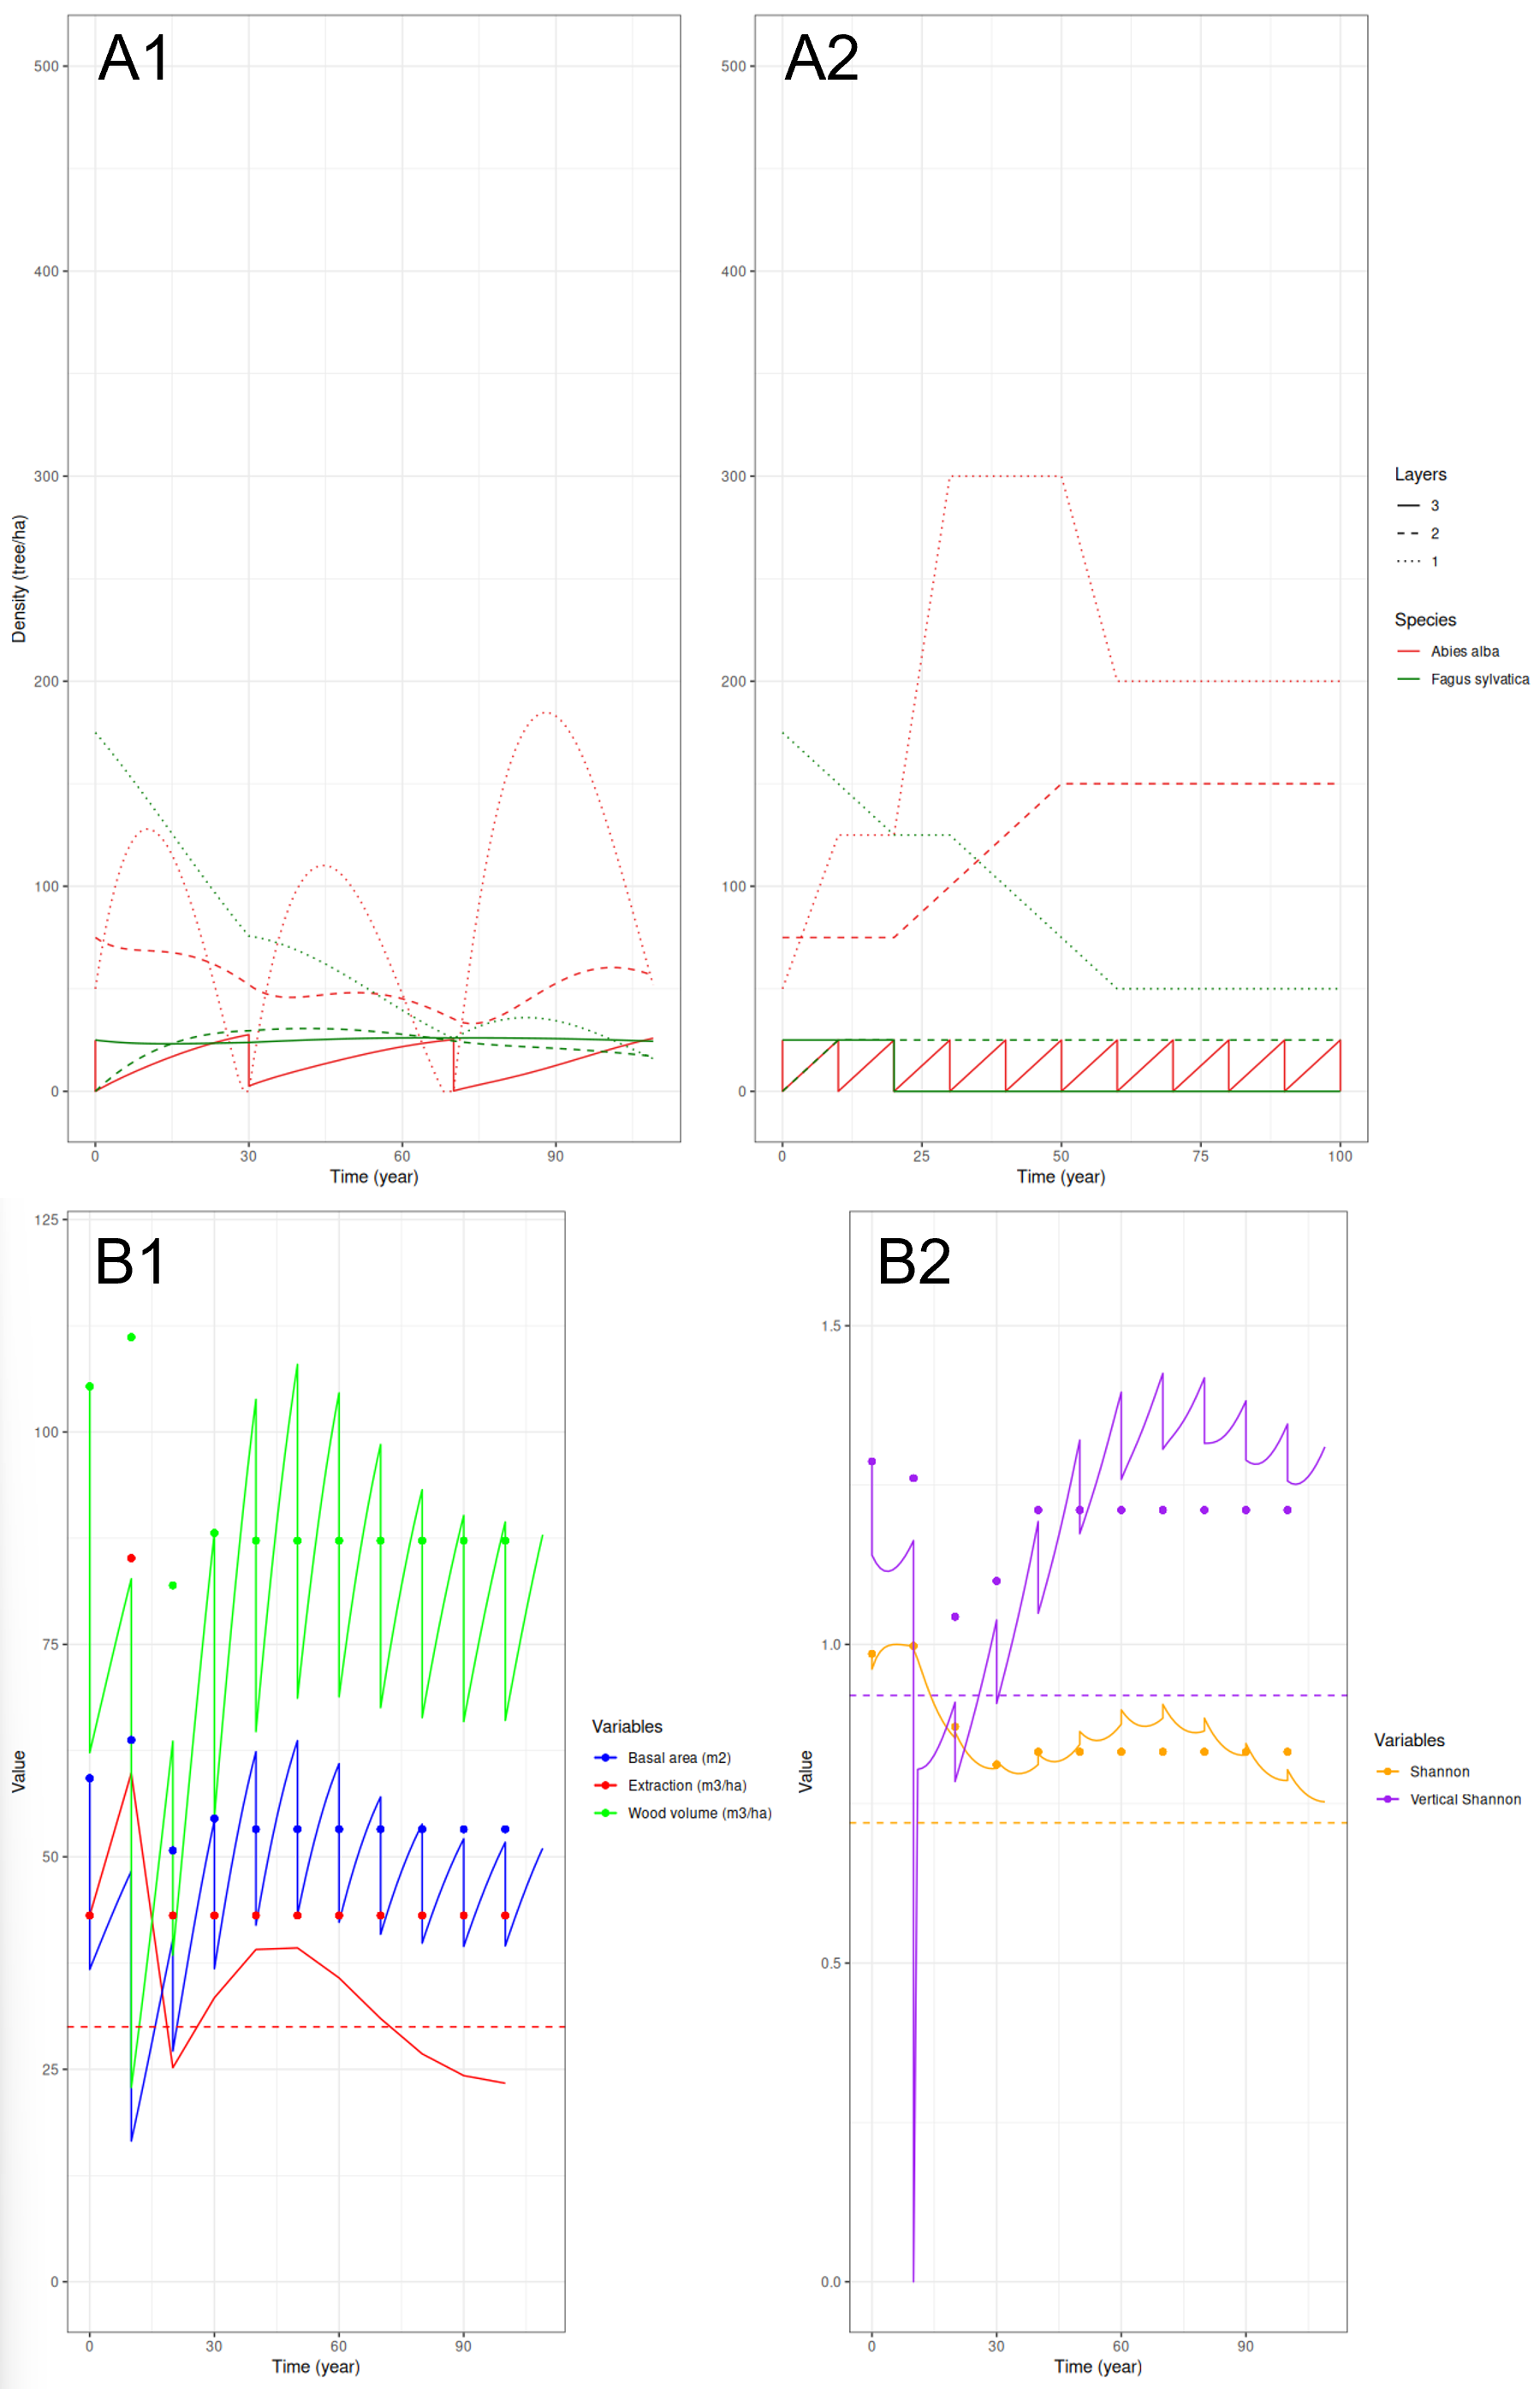
\includegraphics[height=0.9\textheight]{Figure/Results/Extraction_2.png}
    \caption{\underline{Trajectory of one critical state under wood extraction constraints and associated metrics,}
    \underline{with application of control as extraction}. See caption of Figure \ref{fig:Extraction} for details.}
    \label{fig:Extraction2}
\end{figure}

\begin{figure}[b]
    \centering
    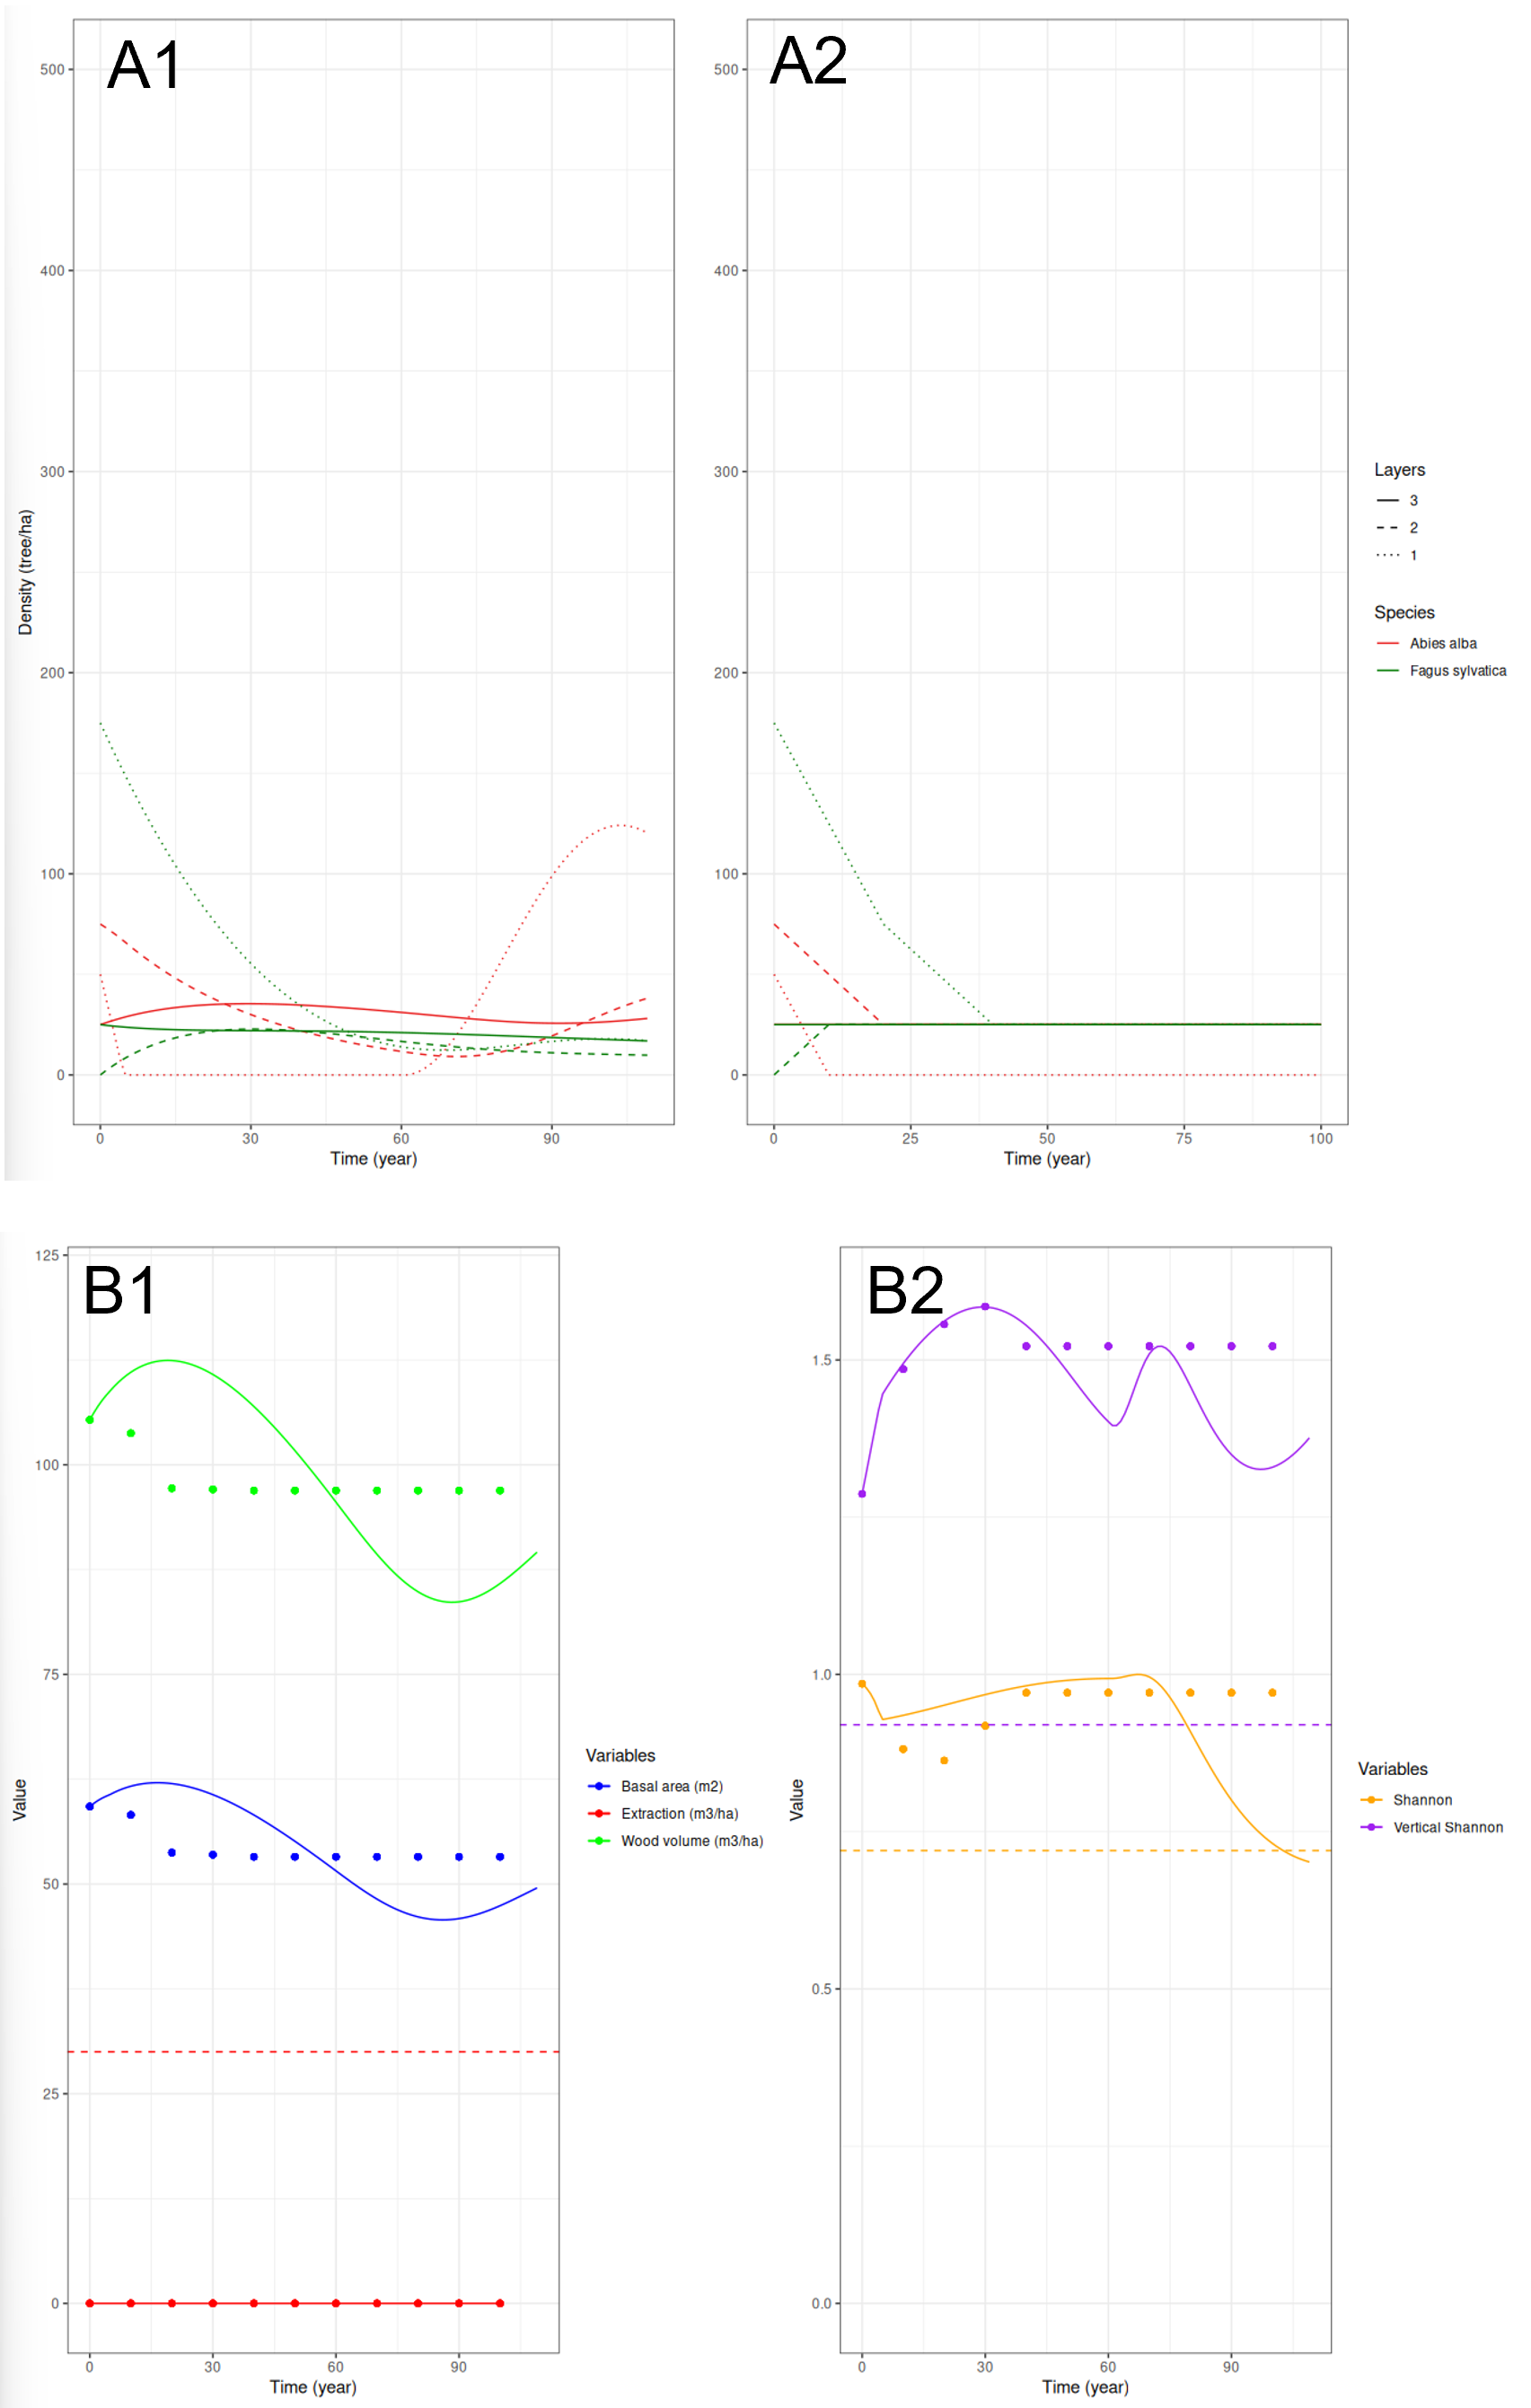
\includegraphics[height=0.9\textheight]{Figure/Results/Diversity_2.png}
    \caption{\underline{Trajectory of one critical state under diversity constraints and associated metrics, with } \underline{application of control as extraction}. See caption of Figure \ref{fig:Extraction} for details.}
    \label{fig:Diversity2}
\end{figure}

\end{document}